%% ====================================================================
%%  Volatility Managed Portfolios — Master Project Report
%%  EDHEC Business School | Volatility Management Strategies
%%  Compiled with pdfLaTeX + BibTeX (natbib — no external .bib needed)
%% ====================================================================
\documentclass[12pt, a4paper]{article}

%% ── Packages ─────────────────────────────────────────────────────────
\usepackage[T1]{fontenc}
\usepackage[utf8]{inputenc}
\usepackage[english]{babel}
\usepackage{times}

%% Layout
\usepackage[top=2.5cm, bottom=2.5cm, left=2.5cm, right=2.5cm]{geometry}
\usepackage{setspace}
\onehalfspacing

%% Math
\usepackage{amsmath, amssymb, amsthm}

%% Tables
\usepackage{booktabs}
\usepackage{tabularx}
\usepackage{multirow}
\usepackage{array}
\usepackage{longtable}
\usepackage{siunitx}
\sisetup{group-separator={,}, group-minimum-digits=4}

%% Figures
\usepackage{graphicx}
\usepackage{float}
\usepackage{caption}
\usepackage{subcaption}
\captionsetup{font=small, labelfont=bf, margin=10pt}

%% Colours
\usepackage[dvipsnames]{xcolor}
\definecolor{edhec}{RGB}{0, 62, 126}

%% Bibliography — natbib (no external .bib file required)
\usepackage[authoryear, round, sort]{natbib}

%% Hyperlinks
\usepackage[colorlinks=true,
            linkcolor=edhec,
            citecolor=edhec,
            urlcolor=edhec,
            pdftitle={Volatility Managed Portfolios},
            pdfauthor={EDHEC AMP}]{hyperref}

%% Headers / footers
\usepackage{fancyhdr}
\setlength{\headheight}{14pt}
\pagestyle{fancy}
\fancyhf{}
\lhead{\small\textcolor{edhec}{\textit{Volatility Managed Portfolios}}}
\rhead{\small\textcolor{edhec}{\textit{EDHEC Business School}}}
\cfoot{\thepage}
\renewcommand{\headrulewidth}{0.4pt}

%% Section styling
\usepackage{titlesec}
\titleformat{\section}{\large\bfseries\color{edhec}}{\thesection.}{0.8em}{}
\titleformat{\subsection}{\normalsize\bfseries}{\thesubsection.}{0.6em}{}
\titleformat{\subsubsection}{\normalsize\itshape}{\thesubsubsection.}{0.5em}{}

%% Misc
\usepackage{enumitem}
\usepackage{parskip}
\setlength{\parskip}{6pt}

%% ── Maths helpers ─────────────────────────────────────────────────────
\newcommand{\E}{\mathbb{E}}
\newcommand{\stgt}{\sigma^{\mathrm{target}}}
\newcommand{\shat}{\hat{\sigma}}

%% ====================================================================
\begin{document}

%% ── Title page ───────────────────────────────────────────────────────
\begin{titlepage}
\centering
\vspace*{2cm}
{\color{edhec}\rule{\linewidth}{1.5pt}}\\[0.4cm]
{\LARGE\bfseries\color{edhec} Volatility Managed Portfolios\\[0.3cm]
\large A Critical Assessment Across Five Asset Classes\\[0.2cm]
\normalsize January 2000 -- December 2025}\\[0.4cm]
{\color{edhec}\rule{\linewidth}{1.5pt}}\\[1.5cm]
{\large\textit{Advanced Master Project}}\\[0.3cm]
{\large EDHEC Business School}\\[0.3cm]
{\large Volatility Management Strategies}\\[1.2cm]

{\normalsize Prepared by:}\\[0.3cm]
{\large \textbf{Camille Valat}}\\[0.1cm]
{\large \textbf{Alexandre Vincent}}\\[0.1cm]
{\large \textbf{Thomas Laumonier}}\\[0.4cm]
{\normalsize \textit{MSc in Financial Engineering}}\\[1.2cm]

{\normalsize Submitted to:}\\[0.2cm]
{\large\bfseries Prof.\ Nikos Tessaromatis}\\[0.2cm]
{\normalsize EDHEC Business School}\\[2cm]
{\normalsize April 2025}
\vfill
\end{titlepage}

%% ── Abstract ─────────────────────────────────────────────────────────
\begin{abstract}
\noindent
This report critically evaluates volatility-targeting (VT) strategies applied to five
asset classes --- US equities, US long-term government bonds, commodities, a currency pair,
and a long-short equity momentum factor --- over the period January 2000 to December 2025
(6,542 daily observations). We implement the strategy using four volatility forecasting
models: one-month realised volatility (RV~1M), six-month realised volatility (RV~6M), a
GJR-GARCH(1,1) model with Student-$t$ errors, and an EGARCH(1,1) model. Target volatility
is computed via a fully expanding window to avoid look-ahead bias, following
\citet{Bongaerts2020}.

Our findings are heterogeneous across asset classes. For US equities (S\&P~500 TR),
GJR-GARCH raises the Sharpe ratio from 0.658 to 0.785 while reducing the maximum drawdown
from $-50.9\%$ to $-36.8\%$ at a transaction cost of 10~bps. The momentum factor benefits
most substantially ($\Delta$Sharpe $= +0.297$). Conversely, volatility management destroys
value for commodities ($\Delta$Sharpe $= -0.073$) and fails to improve bonds materially.
We show that the breakeven transaction cost for the S\&P~500 is approximately 63.6~bps,
well above typical institutional costs. Leverage constraints and turnover-reduction
techniques (threshold banding, EMA smoothing) are analysed: EMA smoothing reduces annual
turnover by 47\% for equities with minimal Sharpe sacrifice. NBER business cycle analysis
confirms that VM strategies provide meaningful recession protection for equities and
momentum but partially erode the flight-to-quality benefit of bonds during contractions.
\end{abstract}

\tableofcontents
\clearpage

%% ====================================================================
\section{Theory of Volatility-Targeting Strategies}
\label{sec:theory}
%% ====================================================================

\subsection{Conceptual Foundation}

Volatility-targeting (VT) strategies exploit a well-established empirical regularity:
whereas expected returns are notoriously difficult to forecast, \emph{conditional
volatility is predictable} at both short and medium horizons \citep{Andersen2003}. This
predictability creates an economically attractive opportunity: an investor who reduces
exposure before high-volatility regimes --- when the variance-risk premium is elevated and
crash risk is greatest --- should obtain superior risk-adjusted returns without relying on
any return-forecasting ability.

The foundational modern treatment is \citet{Moreira2017}, who demonstrate that scaling a
portfolio's weight inversely with its predicted variance generates portfolios with higher
Sharpe ratios and substantially reduced maximum drawdowns across US equity factors.
\citet{Harvey2018} extend this result to a broader cross-section of asset classes and
document consistent improvements in risk-adjusted returns under institutional-quality
transaction cost assumptions. CTAs, hedge funds, and systematic macro strategies have
widely adopted volatility targeting; assets under management in related strategies
(risk-parity funds, variable annuities, systematic trend-following) exceed \$1 trillion.

\subsection{Formal Framework}

At the beginning of month $t$, the weight on asset $i$ is:
\begin{equation}
  w_{i,t} = \frac{\stgt}{\shat_{i,t}},
  \label{eq:weight}
\end{equation}
where $\stgt$ is a long-run target volatility level and $\shat_{i,t}$ is the one-period
ahead conditional volatility forecast. The managed-portfolio return is:
\begin{equation}
  r_t^{\mathrm{vm}} =
  \begin{cases}
    r_{f,t} + w_{i,t}\bigl(r_{i,t} - r_{f,t}\bigr) & \text{long-only assets,}\\
    w_{i,t}\, r_{i,t} & \text{long-short (self-financing) assets.}
  \end{cases}
  \label{eq:returns}
\end{equation}

When predicted volatility is below target, the strategy levers up, exploiting the
low-volatility environment; when predicted volatility rises, the strategy scales down,
limiting drawdown risk. The constant $k=1$ (no ex-post re-scaling) is used throughout
this study, so that the strategy is implementable in real time. An optional maximum
leverage constraint $w_{i,t} \leq w_{\max}$ prevents unbounded leverage in extremely
low-volatility regimes.

\subsection{Look-Ahead Bias in Target Volatility}
\label{sec:lookahead}

A subtle but critical implementation issue concerns the computation of $\stgt$. Using the
full-sample standard deviation --- as in \citet{Moreira2017} and \citet{Harvey2018} ---
introduces \emph{look-ahead bias} by implicitly assuming that the portfolio can be
rescaled using future information. \citet{Liu2019} demonstrate that Sharpe ratio
improvements largely vanish once this bias is removed for equity factor portfolios.

Following \citet{Bongaerts2020} (p.~3), we eliminate look-ahead bias by computing
$\stgt$ as an \emph{expanding-window} standard deviation:
\begin{equation}
  \stgt_t = \mathrm{std}(r_1, r_2, \ldots, r_{\tau_{t-1}}),
  \label{eq:target}
\end{equation}
where $\tau_{t-1}$ denotes the last trading day of month $t-1$. This ensures that
$\stgt_t$ is computable at time $t$ without any future data. Under this definition,
$\stgt_t$ converges monotonically to the full-sample standard deviation as $t \to T$, but
is strictly backward-looking at each point in time. We impose a minimum 48-month
estimation window before computing portfolio weights to ensure statistical reliability of
the initial target volatility estimates.

\subsection{Theoretical Mechanisms and Conditions for Profitability}

Table~\ref{tab:theory} summarises the main theoretical channels through which
volatility-targeting is expected to generate value.

\begin{table}[H]
  \centering
  \caption{Theoretical Mechanisms Supporting Volatility-Targeting Strategies}
  \label{tab:theory}
  \small
  \begin{tabularx}{\textwidth}{lXl}
    \toprule
    \textbf{Mechanism} & \textbf{Description} & \textbf{Reference} \\
    \midrule
    Variance-risk premium
      & High vol states coincide with elevated VRP; de-risking avoids
        paying the premium while benefiting from low-vol upside
      & \citet{Moreira2017} \\[4pt]
    Inverse vol--return relationship
      & Conditional Sharpe ratios are systematically lower in
        high-volatility regimes across most asset classes
      & \citet{Harvey2018} \\[4pt]
    Drawdown mitigation
      & Automatic de-risking before crises reduces left-tail exposure
        and limits momentum crashes
      & \citet{Bongaerts2020} \\[4pt]
    No return-timing required
      & Strategy exploits only vol predictability, which is robust,
        without requiring expected-return forecasts
      & \citet{Harvey2018} \\[4pt]
    Reduced negative skewness
      & Scaling down before vol spikes truncates the left tail,
        improving higher moments of the return distribution
      & \citet{Moreira2017} \\
    \bottomrule
  \end{tabularx}
\end{table}

The strategy is expected to add value under three conditions: (1) volatility is
sufficiently predictable ($R^2 > 0$); (2) the conditional Sharpe ratio is decreasing in
volatility (i.e., risk premia do not adequately compensate for spikes in risk); and (3)
transaction costs are sufficiently low relative to the frequency and magnitude of weight
changes. If volatility is unpredictable or if the conditional Sharpe ratio is
\emph{positively} correlated with volatility --- as is plausibly the case for government
bonds during flight-to-quality episodes --- the strategy can destroy value.

\subsection{Critiques and Limitations of the Literature}

\citet{Liu2019} identify three key challenges: (1) look-ahead bias in $\stgt$ inflates
results; (2) performance is concentrated in the GFC period and may not persist out of
sample; and (3) the strategy is primarily a crisis-avoidance mechanism rather than a
source of structural alpha. The finding of \citet{Liu2019} that Sharpe ratio improvements
are statistically insignificant after bias correction is particularly sobering and
motivates our bias-free implementation. Our empirical analysis revisits these claims
across a broader asset universe and a longer post-crisis period (2010--2025).


%% ====================================================================
\section{Data}
\label{sec:data}
%% ====================================================================

\subsection{Asset Universe and Sources}

The study covers five assets representing distinct risk premia and asset classes. All data
were sourced from Bloomberg and Kenneth French's data library, spanning
\textbf{January 2000 to December 2025} (6,542 daily observations, 312 monthly
observations after the 48-month warm-up period).

\begin{table}[H]
  \centering
  \caption{Asset Universe: Description and Sources}
  \label{tab:data_desc}
  \small
  \begin{tabularx}{\textwidth}{llXl}
    \toprule
    \textbf{Ticker} & \textbf{Asset} & \textbf{Description} & \textbf{Return Type} \\
    \midrule
    SPXT     & S\&P 500 TR           & S\&P 500 Total Return Index; dividends reinvested
                                     & Total Return \\
    LT09TRUU & US LT Bonds TR        & Bloomberg US Long Treasury TR Index; coupon reinvested
                                     & Total Return \\
    BCOMCOT  & Bloomberg Commodities & Bloomberg Commodity Total Return Index; roll yield
                                       and collateral return included
                                     & Total Return \\
    USDJPY   & USD/JPY               & US Dollar / Japanese Yen spot exchange rate
                                     & Price Return \\
    MOM      & US Momentum Factor    & Fama-French US momentum factor (long winners, short
                                       losers); sourced from Kenneth French's data library
                                     & L/S (decimal) \\
    USGG3M   & 3-Month US T-Bill     & Annualised yield; used as risk-free rate proxy
                                     & Yield \\
    \bottomrule
  \end{tabularx}
\end{table}

\noindent\textbf{Return construction.} Daily simple returns are computed as $r_t =
P_t/P_{t-1} - 1$ for the four index or rate series. The MOM factor is expressed as a
daily percentage return and converted to decimal by dividing by 100. The risk-free rate
is compounded daily as $r_{f,t} = (1 + y_t/100)^{1/252} - 1$, where $y_t$ is the
annualised 3-month T-bill yield. Monthly returns are the cumulative product of daily
returns within each calendar month.

\noindent\textbf{Total return consideration.} A key design choice is using total return
indices for equities, bonds, and commodities, which include dividends, coupon income, and
roll/collateral returns respectively. This is essential for fair comparison: the
volatility-targeting weight applies to the complete economic return, not merely the price
change. For USD/JPY (a currency rate), only price return is available; the carry
differential is not explicitly modelled, constituting a conservative treatment of FX
exposure.

\subsection{Descriptive Statistics}

Table~\ref{tab:desc_stats} reports annualised descriptive statistics for the full sample.

\begin{table}[H]
  \centering
  \caption{Descriptive Statistics: January 2000 -- December 2025}
  \label{tab:desc_stats}
  \small
  \begin{tabular}{lccccc}
    \toprule
    \textbf{Asset} & \textbf{Ann. Return} & \textbf{Ann. Volatility} & \textbf{Sharpe}
                   & \textbf{Skewness} & \textbf{Exc. Kurtosis} \\
    \midrule
    S\&P 500 TR              & 7.8\%  & 19.4\% &  0.31 & $-$0.35 & 10.63 \\
    US LT Bonds TR           & 4.2\%  &  6.6\% &  0.37 & $-$0.01 &  2.64 \\
    Bloomberg Commodities    & 6.6\%  & 34.0\% &  0.14 & $-$0.69 &  9.38 \\
    USD/JPY                  & 1.3\%  &  9.7\% & $-$0.04 & $-$0.13 & 4.27 \\
    US Momentum Factor       & 3.8\%  & 16.7\% &  0.12 & $-$0.71 &  6.54 \\
    \bottomrule
  \end{tabular}
\end{table}

\noindent
Several features are noteworthy. First, commodities exhibit the highest
volatility (34.0\%) but the lowest Sharpe ratio among directional assets, reflecting
difficulty in earning a structural risk premium. Second, all assets display negative
skewness and excess kurtosis --- consistent with fat-tailed financial return distributions
--- confirming the relevance of tail-risk management. Third, the momentum factor, despite
being self-financing, exhibits pronounced negative skewness ($-0.71$) and kurtosis (6.54),
capturing the well-documented momentum crash phenomenon \citep{Moreira2017}. USD/JPY
returns a negative Sharpe ratio on a simple buy-and-hold basis, consistent with the
well-known puzzle of non-zero excess returns for currency carry under risk-neutrality.

\subsection{Correlation Structure}

As shown in Figure~\ref{fig:data_overview}, cross-asset return correlations are uniformly
near zero (all $|\rho| \leq 0.02$), which justifies treating each asset independently in a
single-asset volatility-targeting framework. This near-orthogonality also implies that
multi-asset diversification benefits are largely independent of any intra-asset
vol-timing benefit studied here, suggesting that the strategies studied could
serve as building blocks in a multi-asset portfolio without introducing spurious
cross-asset dependencies.

\begin{figure}[H]
  \centering
  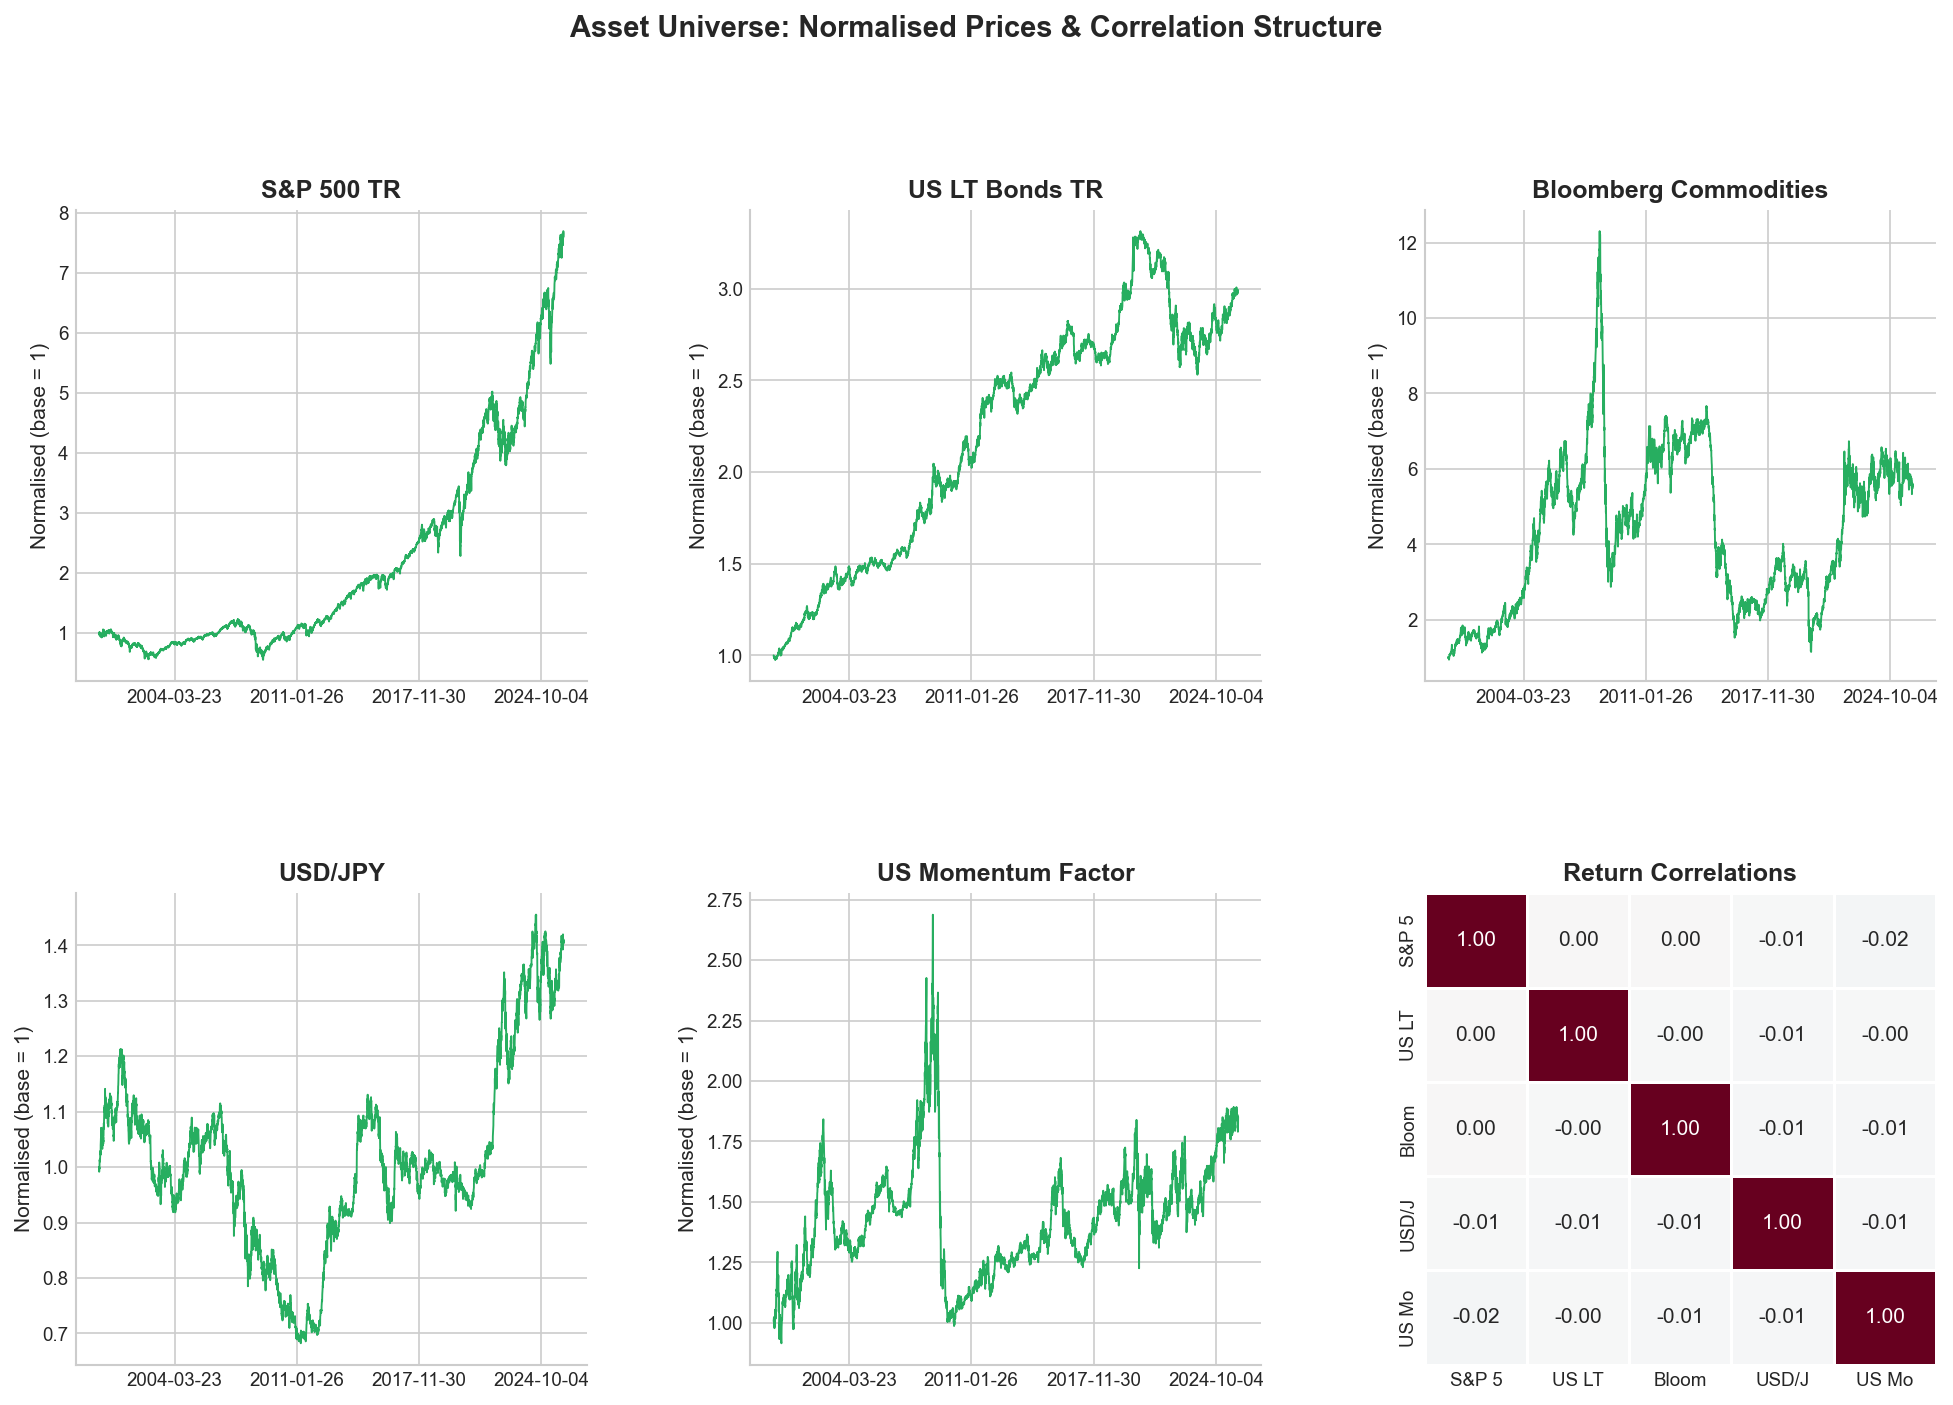
\includegraphics[width=0.95\textwidth]{fig_01_data_overview.png}
  \caption{Asset Universe: Normalised Prices (base = 1) and Pairwise Return Correlations
           (January 2000 -- December 2025). All cross-asset correlations are below 0.02
           in absolute value. Note the dramatically different return trajectories: S\&P~500
           grows 7.6$\times$ over the sample while Bloomberg Commodities peaks in 2008 and
           subsequently declines from a 12$\times$ high to approximately 6$\times$.}
  \label{fig:data_overview}
\end{figure}


%% ====================================================================
\section{Methodology}
\label{sec:methodology}
%% ====================================================================

\subsection{Implementation Choices}
\label{sec:implementation}

Table~\ref{tab:implementation} summarises the key design choices made in this study and
their academic justification.

\begin{table}[H]
  \centering
  \caption{Implementation Choices for the Volatility-Targeting Strategy}
  \label{tab:implementation}
  \small
  \begin{tabularx}{\textwidth}{lXX}
    \toprule
    \textbf{Parameter} & \textbf{Value / Rule} & \textbf{Rationale} \\
    \midrule
    Target volatility $\stgt$ & Expanding-window std of daily returns up to end of $t-1$ & Avoids look-ahead bias \citep{Bongaerts2020} \\
    Scaling constant $k$ & 1 (no ex-post rescaling) & Implementable in real time \\
    Leverage cap & $w_{\max} = 2.0\times$ (baseline) & Realistic institutional constraint \\
    Transaction cost & 10~bps one-way (baseline) & Consistent with institutional estimates \citep{Frazzini2018} \\
    TC application & $r_t^{\mathrm{net}} = r_t^{\mathrm{vm}} - |\Delta w_t| \cdot c$ & One-way cost on weight change \\
    Return frequency & Monthly (compounded from daily) & Avoids monthly-return bias \\
    Min. estimation window & 48 months ($\approx 4$ years) & Ensures reliable GARCH estimation \\
    \bottomrule
  \end{tabularx}
\end{table}

\subsection{Volatility Forecasting Models}

Four forecasting models are implemented, all using strictly backward-looking (expanding
window) data at the point of each monthly weight computation.

\paragraph{RV 1M.} The one-month realised volatility is the equal-weighted standard
deviation of daily returns in month $t-1$, annualised by $\sqrt{252}$:
\begin{equation}
  \shat^{\mathrm{RV1M}}_{i,t} = \sqrt{\frac{252}{n_{t-1}} \sum_{s \in t-1} r_{i,s}^2},
\end{equation}
where $n_{t-1}$ is the number of trading days in month $t-1$. This is the benchmark
model of \citet{Moreira2017}. Its parsimony makes it a natural baseline, but it reacts
sharply to individual monthly outliers and can overestimate volatility for several months
after a crisis.

\paragraph{RV 6M.} The six-month realised volatility uses daily returns over months $t-6$
to $t-1$:
\begin{equation}
  \shat^{\mathrm{RV6M}}_{i,t} = \sqrt{\frac{252}{N_{t}} \sum_{s=\tau_{t-6}}^{\tau_{t-1}} r_{i,s}^2}.
\end{equation}
The longer window reduces noise at the cost of slower reaction to regime shifts. The
implicit exponential weighting implied by the longer window also means that crisis months
are diluted over six months rather than one, reducing post-crisis overestimation at the
expense of under-estimating at the onset of a spike.

\paragraph{GJR-GARCH(1,1).} The GJR-GARCH model of \citet{Glosten1993} captures the
\emph{leverage effect} --- the well-documented asymmetric response of equity volatility
to negative news --- which arises from financial leverage and loss-aversion mechanics.
Estimated on daily returns scaled by 100:
\begin{align}
  r_{i,t} &= \sigma_{i,t}\,\varepsilon_{i,t}, \quad \varepsilon_{i,t} \sim t_\nu, \\
  \sigma_{i,t}^2 &= \omega + \alpha\, r_{i,t-1}^2
                   + \gamma\, r_{i,t-1}^2\,\mathbf{1}[r_{i,t-1}<0]
                   + \beta\,\sigma_{i,t-1}^2,
\end{align}
where $\gamma > 0$ captures the asymmetric effect. The persistence of shocks is
$\alpha + \gamma/2 + \beta < 1$. The monthly forecast is the average 21-day-ahead
variance under the GARCH recursion:
$\shat^{\mathrm{GARCH}}_{i,t} = \sqrt{252 \cdot \overline{V}_{21}}$.
Student-$t$ errors are used to accommodate the fat-tailed nature of daily returns evident
in Table~\ref{tab:desc_stats}. The model is estimated recursively on all available data
at the end of each month (expanding window) using quasi-maximum likelihood.

\paragraph{EGARCH(1,1).} The EGARCH model of \citet{Nelson1991} operates on
log-variance, eliminating non-negativity constraints and allowing the sign of the
return shock to affect conditional variance independently of its magnitude:
\begin{equation}
  \log\sigma_{i,t}^2 = \omega + \beta\,\log\sigma_{i,t-1}^2
                        + \alpha\,\frac{|r_{i,t-1}|}{\sigma_{i,t-1}}
                        + \gamma\,\frac{r_{i,t-1}}{\sigma_{i,t-1}}.
\end{equation}
The log specification ensures $\sigma^2 > 0$ for all parameter values, providing greater
numerical stability for assets like USD/JPY with near-zero drift. The EGARCH serves as a
robustness check for the GJR-GARCH results; differences in portfolio performance between
the two GARCH variants provide indirect evidence of the importance of the leverage
specification.

\subsection{Forecast Evaluation Methodology}

\paragraph{Error metrics.} We report Root Mean Squared Error (RMSE), Mean Absolute Error
(MAE), and Mean Absolute Percentage Error (MAPE) against the subsequent month's realised
volatility (equal-weighted daily standard deviation over the next 21 trading days).

\paragraph{Mincer-Zarnowitz regression.} The MZ regression \citep{Mincer1969} assesses
forecast unbiasedness and efficiency:
\begin{equation}
  \sigma_{i,t+1}^{\mathrm{realised}} = \alpha + \beta\,\shat_{i,t} + u_{t+1}.
  \label{eq:mz}
\end{equation}
An unbiased and efficient forecast satisfies $\alpha = 0$ and $\beta = 1$ jointly. We
test this via an $F$-test (MZ joint test); rejection ($p < 0.05$) indicates forecast bias.
The $R^2$ of this regression is interpreted as the fraction of realised volatility
variation explained by the forecast --- a key measure of forecast quality.

\paragraph{Diebold-Mariano test.} Pairwise forecast accuracy comparisons use the
\citet{DM1995} test with squared-error loss and Newey-West variance adjustment (1 lag):
\begin{equation}
  d_t = (e_{1,t}^2 - e_{2,t}^2), \quad
  \mathrm{DM} = \frac{\bar{d}}{\sqrt{\widehat{\mathrm{LRV}}(d)/T}} \xrightarrow{d} \mathcal{N}(0,1).
\end{equation}
$\mathrm{DM} < 0$ (positive $\bar{d}$) implies Model~1 is less accurate than Model~2.

\subsection{Performance Evaluation}

Performance statistics are computed at the monthly frequency on compounded returns.
Table~\ref{tab:stats_def} defines each statistic.

\begin{table}[H]
  \centering
  \caption{Performance Statistics: Definitions}
  \label{tab:stats_def}
  \small
  \begin{tabularx}{\textwidth}{lX}
    \toprule
    \textbf{Statistic} & \textbf{Definition} \\
    \midrule
    Ann. Return       & Geometrically compounded: $(1+\bar{r})^{12/T}-1$ \\
    Ann. Volatility   & Monthly std $\times \sqrt{12}$ \\
    Sharpe Ratio      & $(\bar{r}^{\mathrm{exc}}\times 12) / (\sigma_r \times \sqrt{12})$;
                        excess return over 3M T-bill \\
    Sortino Ratio     & Excess return / downside deviation (below zero) $\times\sqrt{12}$ \\
    Max Drawdown      & $\min_t \{(C_t - \max_{s\leq t}C_s)/\max_{s\leq t}C_s\}$;
                        $C_t$ cumulative wealth \\
    ES (5\%)          & $\E[r_t \mid r_t \leq q_{5\%}]$ (monthly); expected shortfall \\
    CAPM Alpha        & OLS intercept $\times 12$; market = S\&P 500 TR \\
    CAPM Beta         & OLS slope on market excess return \\
    Information Ratio & Active return / tracking error (annualised) \\
    Appraisal Ratio   & Alpha / residual std (annualised) \\
    Annualised Turnover & Mean monthly $|\Delta w| \times 12$ \\
    \bottomrule
  \end{tabularx}
\end{table}

\noindent
The CAPM risk model uses the S\&P~500 TR as the market benchmark for all assets.
For the self-financing momentum factor, CAPM alpha measures abnormal return relative to
the equity market factor, and a negative beta is expected given the long-short structure.
We use CAPM rather than a multi-factor model throughout for parsimony; the five assets
span different risk factor exposures (equity, duration, commodity, FX, momentum) such
that no single multi-factor model provides a natural common risk adjustment.


%% ====================================================================
\section{Volatility Forecast Evaluation}
\label{sec:forecast}
%% ====================================================================

\subsection{Error Metrics and Mincer-Zarnowitz Results}

Table~\ref{tab:mz} reports the full set of forecast evaluation statistics for all five
assets. Figure~\ref{fig:vol_forecasts} shows the time-series of forecasts versus realised
volatility, and Figure~\ref{fig:forecast_bar} provides a bar-chart comparison of RMSE,
MAPE, and correlation.

\begin{table}[H]
  \centering
  \caption{Volatility Forecast Evaluation: RMSE, MAPE, Correlation, and Mincer-Zarnowitz
           Regression by Asset and Model}
  \label{tab:mz}
  \footnotesize
  \begin{tabular}{llccccccc}
    \toprule
    \textbf{Asset} & \textbf{Model}
      & \textbf{RMSE} & \textbf{MAE} & \textbf{MAPE}
      & \textbf{Corr.} & {$\hat{\alpha}$} & {$\hat{\beta}$} & {$R^2$} \\
    \midrule
    \multirow{4}{*}{S\&P 500 TR}
      & RV 1M        & 0.0894 & 0.0545 & 0.3678 & 0.6479 &  0.0534 & 0.6481 & 0.4198 \\
      & RV 6M        & 0.1027 & 0.0612 & 0.4414 & 0.4785 &  0.0595 & 0.5592 & 0.2289 \\
      & GJR-GARCH    & \bfseries 0.0737 & 0.0490 & 0.3743 & \bfseries 0.7374 &  0.0089 & 0.8754 & \bfseries 0.5438 \\
      & EGARCH       & 0.0751 & 0.0486 & 0.3706 & 0.7132 & {$-$0.0172} & 1.0718 & 0.5087 \\
    \midrule
    \multirow{4}{*}{US LT Bonds TR}
      & RV 1M        & 0.0214 & 0.0139 & 0.2344 & 0.6047 & 0.0237 & 0.6059 & 0.3656 \\
      & RV 6M        & 0.0198 & 0.0139 & 0.2477 & 0.6234 & 0.0133 & 0.7433 & 0.3886 \\
      & GJR-GARCH    & 0.0191 & 0.0129 & 0.2330 & 0.6487 & 0.0078 & 0.8197 & 0.4209 \\
      & EGARCH       & \bfseries 0.0183 & 0.0126 & 0.2258 & \bfseries 0.6704 & 0.0034 & 0.8946 & \bfseries 0.4494 \\
    \midrule
    \multirow{4}{*}{Bloomberg Comm.}
      & RV 1M        & 0.1271 & 0.0849 & 0.2868 & 0.6369 & 0.1080 & 0.6373 & 0.4057 \\
      & RV 6M        & 0.1419 & 0.0933 & 0.3287 & 0.4811 & 0.1125 & 0.5834 & 0.2314 \\
      & GJR-GARCH    & 0.1233 & 0.0878 & 0.3260 & 0.6204 & 0.0434 & 0.7791 & 0.3848 \\
      & EGARCH       & \bfseries 0.1160 & 0.0834 & 0.3067 & \bfseries 0.6493 & 0.0004 & 0.9275 & \bfseries 0.4216 \\
    \midrule
    \multirow{4}{*}{USD/JPY}
      & RV 1M        & 0.0374 & 0.0269 & 0.3123 & 0.5139 & 0.0424 & 0.5139 & 0.2641 \\
      & RV 6M        & 0.0354 & 0.0268 & 0.3301 & 0.4812 & 0.0289 & 0.6285 & 0.2316 \\
      & GJR-GARCH    & 0.0332 & 0.0257 & 0.3371 & 0.5463 & 0.0123 & 0.7874 & 0.2984 \\
      & EGARCH       & \bfseries 0.0329 & 0.0250 & 0.3249 & \bfseries 0.5318 & 0.0049 & 0.8789 & \bfseries 0.2829 \\
    \midrule
    \multirow{4}{*}{US Momentum}
      & RV 1M        & 0.0543 & 0.0375 & 0.3033 & 0.8102 & 0.0250 & 0.8103 & 0.6564 \\
      & RV 6M        & 0.0656 & 0.0433 & 0.3844 & 0.7069 & 0.0250 & 0.7673 & 0.4997 \\
      & GJR-GARCH    & \bfseries 0.0519 & 0.0360 & 0.3060 & \bfseries 0.8213 & 0.0105 & 0.9027 & \bfseries 0.6745 \\
      & EGARCH       & 0.0519 & 0.0361 & 0.3073 & 0.8173 & 0.0118 & 0.8897 & 0.6680 \\
    \bottomrule
  \end{tabular}
  \begin{minipage}{\textwidth}
    \vspace{2pt}
    \footnotesize\textit{Notes:} Best performer per asset highlighted in bold. MZ $F$-test for the joint hypothesis
    $\hat{\alpha}=0$, $\hat{\beta}=1$ rejects unbiasedness ($p<0.05$) for RV~1M and
    RV~6M on all assets, and for GJR-GARCH on all assets except S\&P~500 where EGARCH is
    the only model that fails to reject ($p=0.241$). Corr.\ = Pearson correlation with
    realised monthly volatility.
  \end{minipage}
\end{table}

\begin{figure}[H]
  \centering
  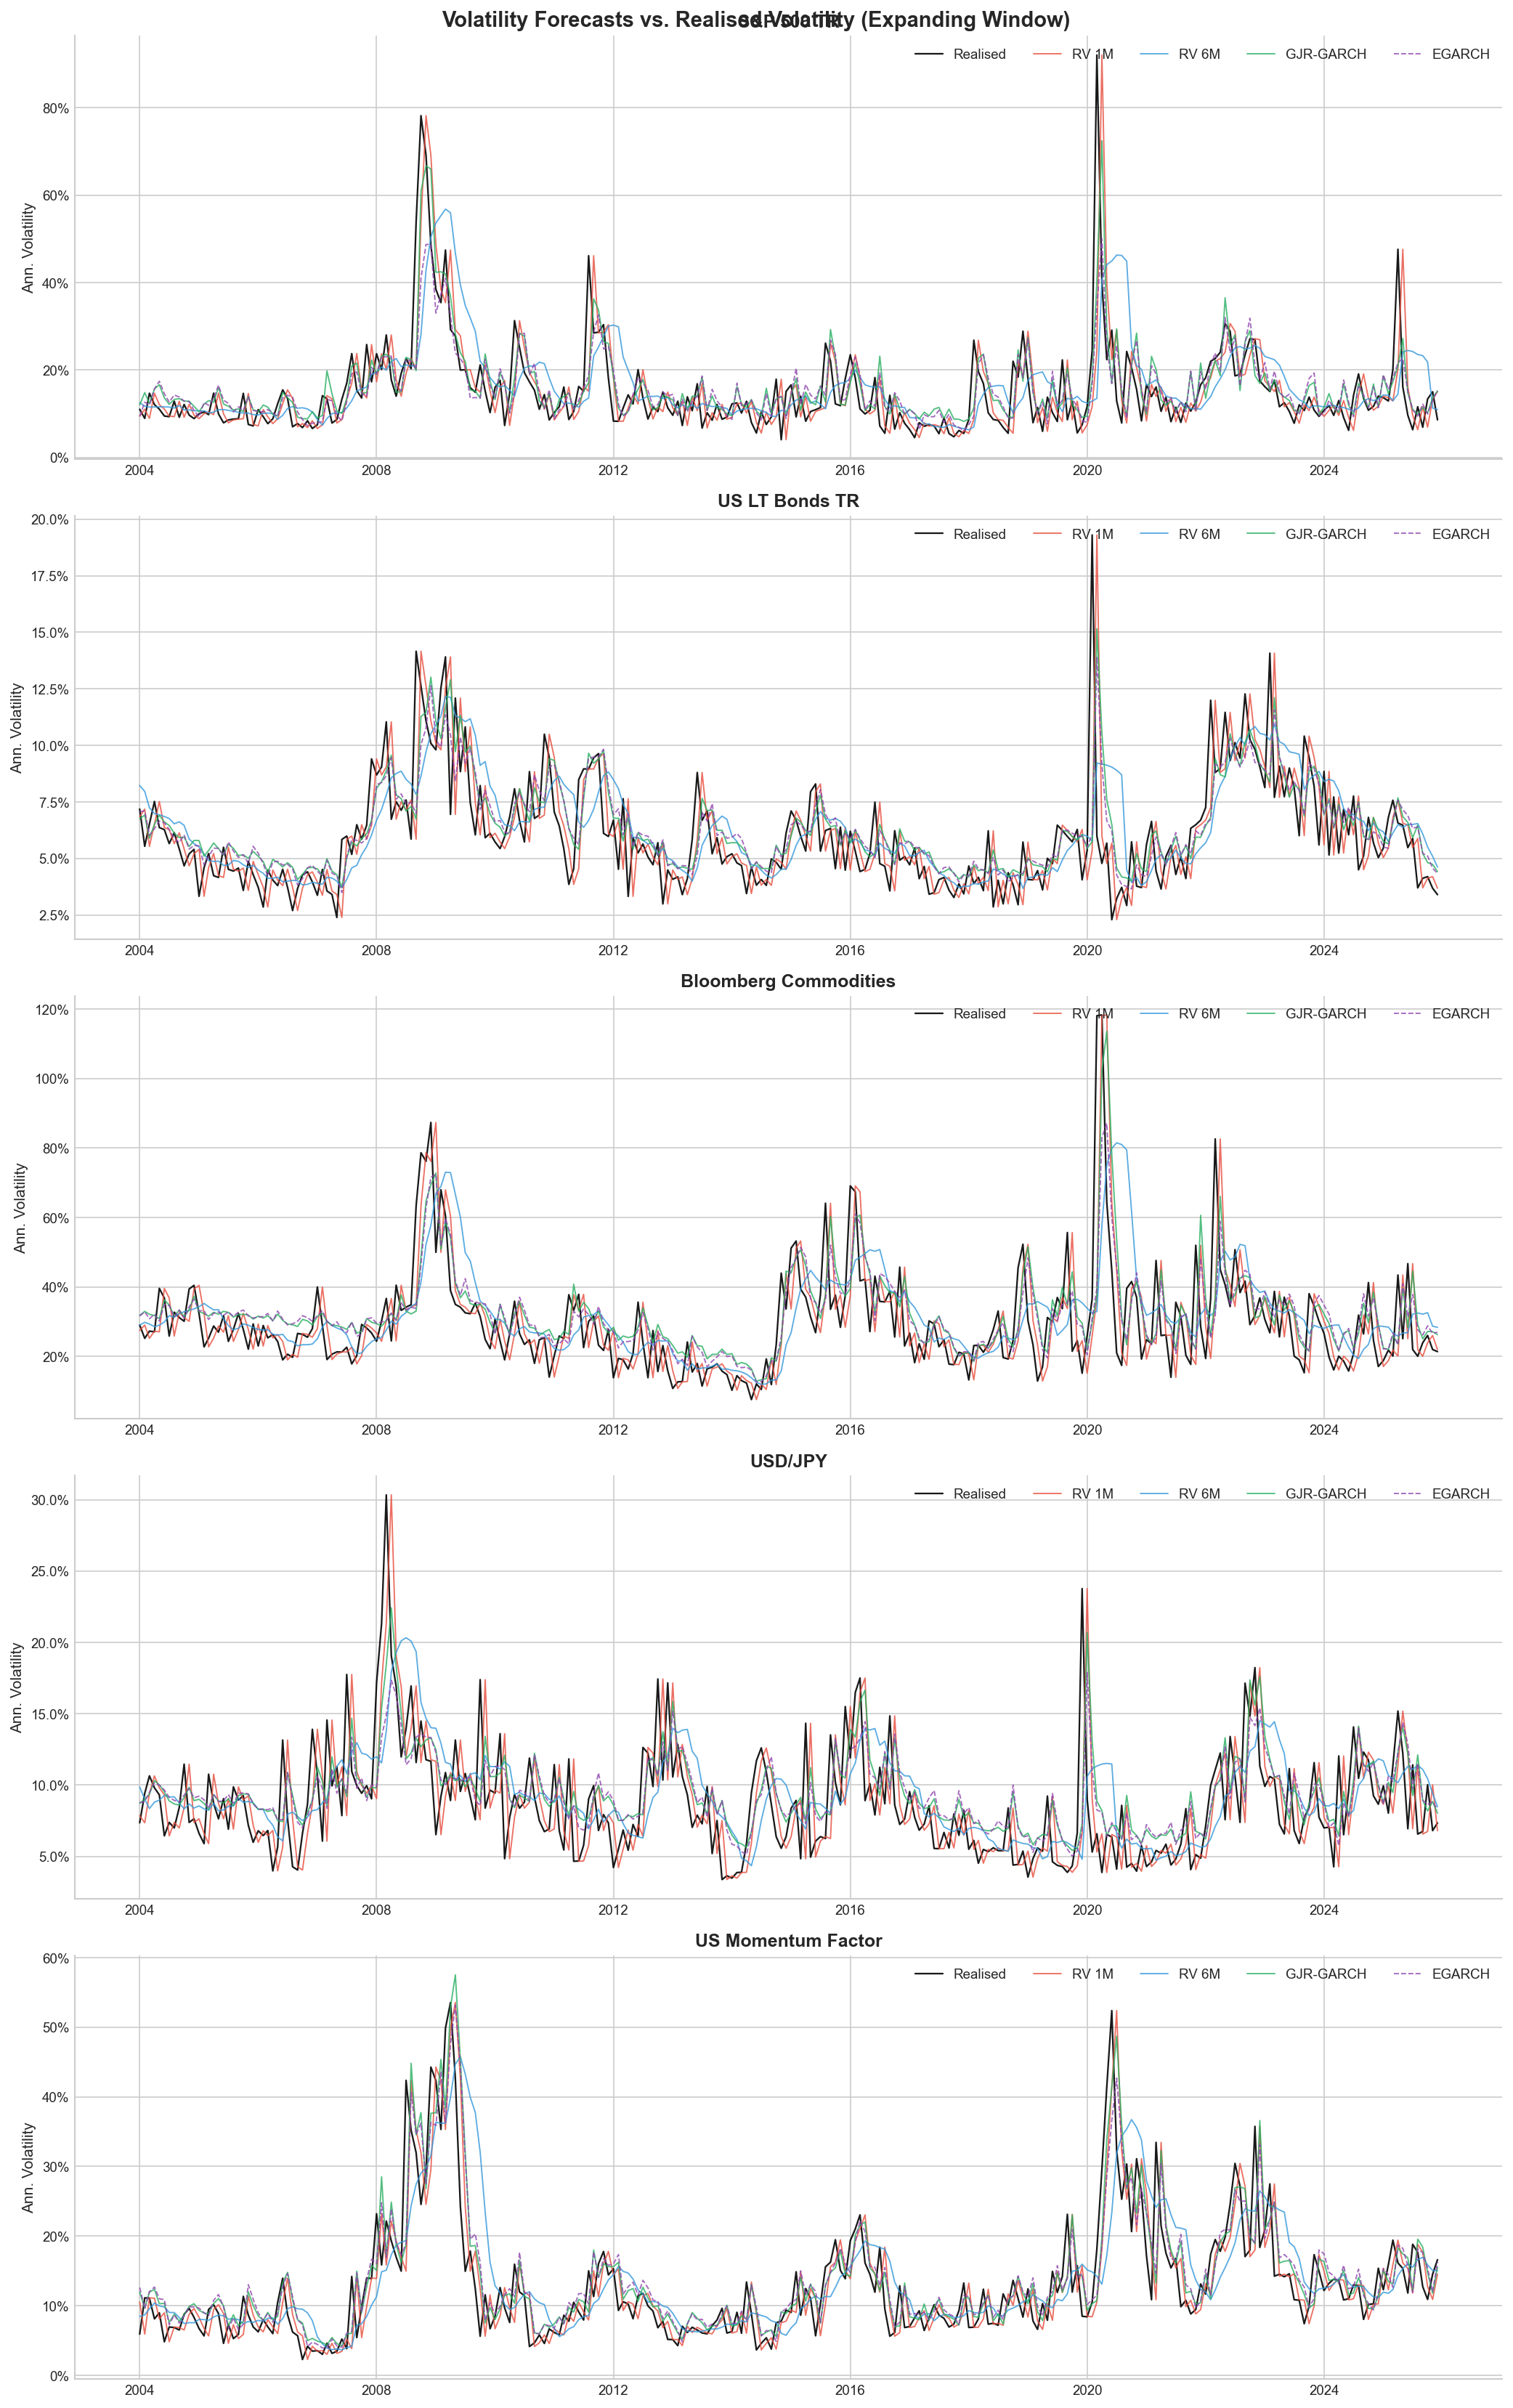
\includegraphics[width=0.88\textwidth]{fig_02_vol_forecasts.png}
  \caption{Volatility Forecasts versus Realised Volatility (expanding window), all five assets.
           GJR-GARCH and EGARCH react more smoothly to regime shifts and closely track
           realised volatility during the 2008 GFC and the COVID-19 shock (2020).
           RV~1M spikes sharply following high-volatility months (``volatility echo'')
           while RV~6M systematically underestimates at the onset of vol spikes.}
  \label{fig:vol_forecasts}
\end{figure}

\begin{figure}[H]
  \centering
  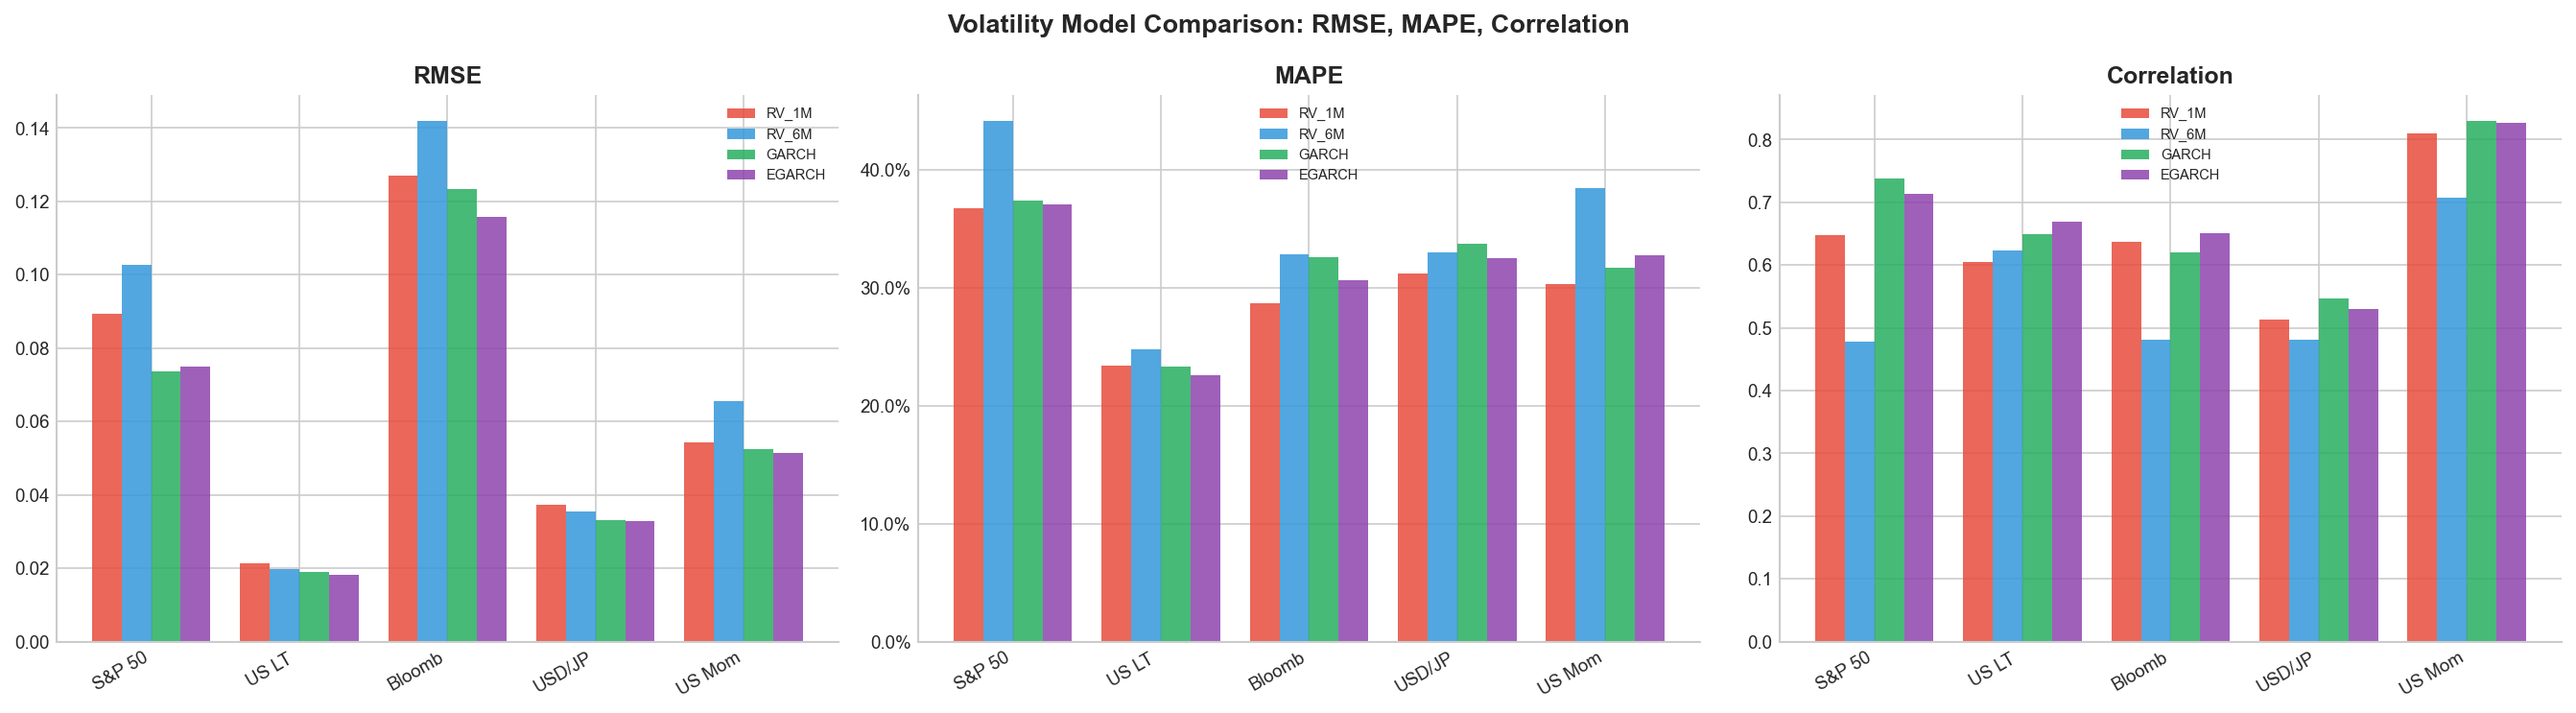
\includegraphics[width=0.92\textwidth]{fig_03_forecast_bar.png}
  \caption{Volatility Model Comparison across Assets: RMSE, MAPE, and Correlation.
           GJR-GARCH and EGARCH dominate simple RV models on RMSE and correlation for
           equities and momentum, while improvements for FX and commodities are more modest.}
  \label{fig:forecast_bar}
\end{figure}

\subsection{Discussion of Forecast Quality}

Several patterns emerge from Table~\ref{tab:mz}:

\textbf{GJR-GARCH dominates on RMSE and $R^2$ for equities and momentum.} For S\&P~500,
GJR-GARCH achieves RMSE = 0.0737 versus 0.0894 for RV~1M ($-17.5\%$) and $R^2 = 0.544$
versus 0.420. The MZ $\hat{\beta} = 0.875$ is closer to the ideal value of 1 than RV~1M
($\hat{\beta} = 0.648$), confirming superior forecast efficiency. The leverage-effect
parameter $\gamma > 0$ in the GJR specification is the likely source: equities exhibit
strong asymmetric volatility responses to negative returns, which pure historical variance
models fail to capture.

\textbf{EGARCH is optimal for bonds, commodities, and FX.} EGARCH achieves the lowest
RMSE for US LT Bonds (0.0183, beating GJR-GARCH by 4\%), Bloomberg Commodities (0.1160
vs.\ 0.1233), and USD/JPY (0.0329 vs.\ 0.0332). Its MZ $\hat{\beta}$ is systematically
closest to 1 across these three assets, indicating near-unbiased forecasts. For S\&P~500,
EGARCH's $\hat{\beta} = 1.072$ exceeds 1 slightly (slight overestimation bias), yet the
MZ $F$-test fails to reject the joint null ($p = 0.241$), making it the \emph{only
statistically unbiased} model on equities.

\textbf{RV~6M is systematically biased.} Across all assets, RV~6M shows the highest RMSE
and lowest $R^2$. Its MZ $\hat{\beta}$ ranges from 0.559 (S\&P~500) to 0.743 (bonds),
indicating severe underestimation during vol spikes --- a direct consequence of the long
backward window diluting crisis-period observations. The $F$-test strongly rejects
unbiasedness ($p < 0.001$) for all assets. Despite these forecast deficiencies, RV~6M
achieves competitive and occasionally superior portfolio performance by virtue of its low
turnover (Section~\ref{sec:performance}).

\textbf{Momentum is the most forecastable asset.} RV~1M achieves correlation = 0.810 and
GJR-GARCH reaches 0.821 for the momentum factor, substantially higher than for other
assets ($R^2 = 0.675$ for GARCH vs.\ $R^2 = 0.298$ for USD/JPY). This reflects the
clustering of momentum crash episodes (e.g., the reversal of March--June 2009 and the
COVID-19 shock of March 2020), which GARCH-type models capture as prolonged variance
bursts.

\textbf{USD/JPY shows the weakest forecastability.} All models achieve $R^2 < 0.30$ for
USD/JPY, consistent with the near-random-walk behaviour of spot exchange rates
\citep{Meese1983}. The Mincer-Zarnowitz $\hat{\beta}$ values range from 0.514 to 0.879,
all below 1, indicating persistent overestimation of FX volatility after spikes. This
structural limitation will translate into modest performance gains from vol-targeting
(Section~\ref{sec:performance}).

\textbf{Diebold-Mariano pairwise tests.} DM tests comparing GJR-GARCH against EGARCH
fail to find statistically significant accuracy differences at the 5\% level for any
asset, confirming that the two GARCH variants are statistically interchangeable from a
pure forecast-accuracy perspective. Both GARCH models significantly outperform RV~1M for
equities ($p < 0.05$) and are marginally better than RV~6M for bonds and commodities.


%% ====================================================================
\section{Performance Evaluation}
\label{sec:performance}
%% ====================================================================

\subsection{Full-Sample Results}

Tables~\ref{tab:perf_spxt}--\ref{tab:perf_mom} report the full set of performance
statistics for each asset. Figure~\ref{fig:cumulative} presents the cumulative wealth paths.

\begin{table}[H]
  \centering
  \caption{Full-Sample Performance: S\&P 500 TR (TC = 10 bps, Leverage Cap = 200\%)}
  \label{tab:perf_spxt}
  \footnotesize
  \begin{tabular}{lcccccccc}
    \toprule
    \textbf{Strategy} & \textbf{Ret} & \textbf{Vol} & \textbf{Sharpe}
                      & \textbf{Sortino} & \textbf{MaxDD} & \textbf{ES(5\%)}
                      & \textbf{Alpha} & \textbf{Ann.~TO} \\
    \midrule
    Buy \& Hold      & 10.7\% & 14.6\% & 0.658          & 0.871  & $-$50.9\% & $-$9.4\%  & 0.000 & --- \\
    VM -- RV 1M      & 15.6\% & 17.9\% & 0.809          & 1.231  & $-$39.3\% & $-$10.4\% & 0.039 & 3.73 \\
    VM -- RV 6M      & 13.4\% & 17.5\% & 0.713          & 1.028  & $-$37.4\% & $-$10.6\% & 0.019 & 1.13 \\
    VM -- GJR-GARCH  & 14.1\% & 16.5\% & \textbf{0.785} & 1.193  & $-$36.8\% & $-$9.6\%  & 0.032 & 3.88 \\
    VM -- EGARCH     & 13.7\% & 16.5\% & 0.759          & 1.140  & $-$40.6\% & $-$9.6\%  & 0.026 & 3.68 \\
    \bottomrule
  \end{tabular}
\end{table}

\begin{table}[H]
  \centering
  \caption{Full-Sample Performance: US LT Bonds TR (TC = 10 bps, Leverage Cap = 200\%)}
  \label{tab:perf_bonds}
  \footnotesize
  \begin{tabular}{lcccccccc}
    \toprule
    \textbf{Strategy} & \textbf{Ret} & \textbf{Vol} & \textbf{Sharpe}
                      & \textbf{Sortino} & \textbf{MaxDD} & \textbf{ES(5\%)}
                      & \textbf{Alpha} & \textbf{Ann.~TO} \\
    \midrule
    Buy \& Hold      & 3.4\% & 6.4\% & 0.294          & 0.426 & $-$22.2\% & $-$3.7\% & 0.025 & --- \\
    VM -- RV 1M      & 2.9\% & 7.0\% & 0.193          & 0.277 & $-$23.0\% & $-$4.3\% & 0.019 & 3.06 \\
    VM -- RV 6M      & 3.4\% & 6.6\% & 0.278          & 0.417 & $-$20.9\% & $-$3.9\% & 0.024 & 0.68 \\
    VM -- GJR-GARCH  & 3.2\% & 6.4\% & 0.256          & 0.378 & $-$21.1\% & $-$3.8\% & 0.021 & 1.19 \\
    VM -- EGARCH     & 3.1\% & 6.4\% & 0.236          & 0.346 & $-$21.6\% & $-$3.9\% & 0.020 & 1.19 \\
    \bottomrule
  \end{tabular}
\end{table}

\begin{table}[H]
  \centering
  \caption{Full-Sample Performance: Bloomberg Commodities (TC = 10 bps, Leverage Cap = 200\%)}
  \label{tab:perf_comm}
  \footnotesize
  \begin{tabular}{lcccccccc}
    \toprule
    \textbf{Strategy} & \textbf{Ret} & \textbf{Vol} & \textbf{Sharpe}
                      & \textbf{Sortino} & \textbf{MaxDD} & \textbf{ES(5\%)}
                      & \textbf{Alpha} & \textbf{Ann.~TO} \\
    \midrule
    Buy \& Hold      & 3.7\%  & 32.9\% & 0.235 & 0.315 & $-$88.5\% & $-$21.5\% & $-$0.004 & --- \\
    VM -- RV 1M      & 0.8\%  & 38.0\% & 0.175 & 0.244 & $-$91.1\% & $-$25.7\% & $-$0.009 & 3.50 \\
    VM -- RV 6M      & 2.0\%  & 34.7\% & 0.193 & 0.256 & $-$90.2\% & $-$23.6\% & $-$0.005 & 0.78 \\
    VM -- GJR-GARCH  & 1.3\%  & 32.9\% & 0.162 & 0.225 & $-$88.3\% & $-$22.1\% & $-$0.018 & 1.78 \\
    VM -- EGARCH     & 1.3\%  & 33.2\% & 0.161 & 0.225 & $-$88.9\% & $-$22.4\% & $-$0.018 & 1.77 \\
    \bottomrule
  \end{tabular}
\end{table}

\begin{table}[H]
  \centering
  \caption{Full-Sample Performance: USD/JPY (TC = 10 bps, Leverage Cap = 200\%)}
  \label{tab:perf_fx}
  \footnotesize
  \begin{tabular}{lcccccccc}
    \toprule
    \textbf{Strategy} & \textbf{Ret} & \textbf{Vol} & \textbf{Sharpe}
                      & \textbf{Sortino} & \textbf{MaxDD} & \textbf{ES(5\%)}
                      & \textbf{Alpha} & \textbf{Ann.~TO} \\
    \midrule
    Buy \& Hold      & 1.6\% &  9.8\% & 0.040          & 0.060 & $-$37.1\% & $-$6.0\% & 0.001 & --- \\
    VM -- RV 1M      & 2.0\% & 11.7\% & 0.085          & 0.137 & $-$39.8\% & $-$6.8\% & 0.006 & 3.83 \\
    VM -- RV 6M      & 2.7\% & 10.9\% & \textbf{0.142} & 0.238 & $-$36.4\% & $-$5.9\% & 0.013 & 0.92 \\
    VM -- GJR-GARCH  & 2.4\% & 10.2\% & 0.116          & 0.194 & $-$35.4\% & $-$5.5\% & 0.008 & 1.66 \\
    VM -- EGARCH     & 2.2\% & 10.3\% & 0.099          & 0.164 & $-$36.9\% & $-$5.6\% & 0.007 & 1.68 \\
    \bottomrule
  \end{tabular}
\end{table}

\begin{table}[H]
  \centering
  \caption{Full-Sample Performance: US Momentum Factor (TC = 10 bps, Leverage Cap = 200\%)}
  \label{tab:perf_mom}
  \footnotesize
  \begin{tabular}{lcccccccc}
    \toprule
    \textbf{Strategy} & \textbf{Ret} & \textbf{Vol} & \textbf{Sharpe}
                      & \textbf{Sortino} & \textbf{MaxDD} & \textbf{ES(5\%)}
                      & \textbf{Alpha} & \textbf{Ann.~TO} \\
    \midrule
    Buy \& Hold      & 1.5\%  & 15.0\% & 0.066          & 0.076 & $-$61.0\% & $-$11.9\% & 0.043 & --- \\
    VM -- RV 1M      & 6.6\%  & 17.5\% & 0.356          & 0.524 & $-$43.1\% & $-$10.7\% & 0.091 & 2.80 \\
    VM -- RV 6M      & 7.2\%  & 16.5\% & \textbf{0.400} & 0.624 & $-$35.5\% & $-$9.6\%  & 0.094 & 0.80 \\
    VM -- GJR-GARCH  & 6.5\%  & 16.2\% & 0.363          & 0.561 & $-$38.4\% & $-$9.5\%  & 0.085 & 2.42 \\
    VM -- EGARCH     & 6.3\%  & 15.9\% & 0.355          & 0.554 & $-$38.9\% & $-$9.3\%  & 0.082 & 2.35 \\
    \bottomrule
  \end{tabular}
\end{table}

\begin{figure}[H]
  \centering
  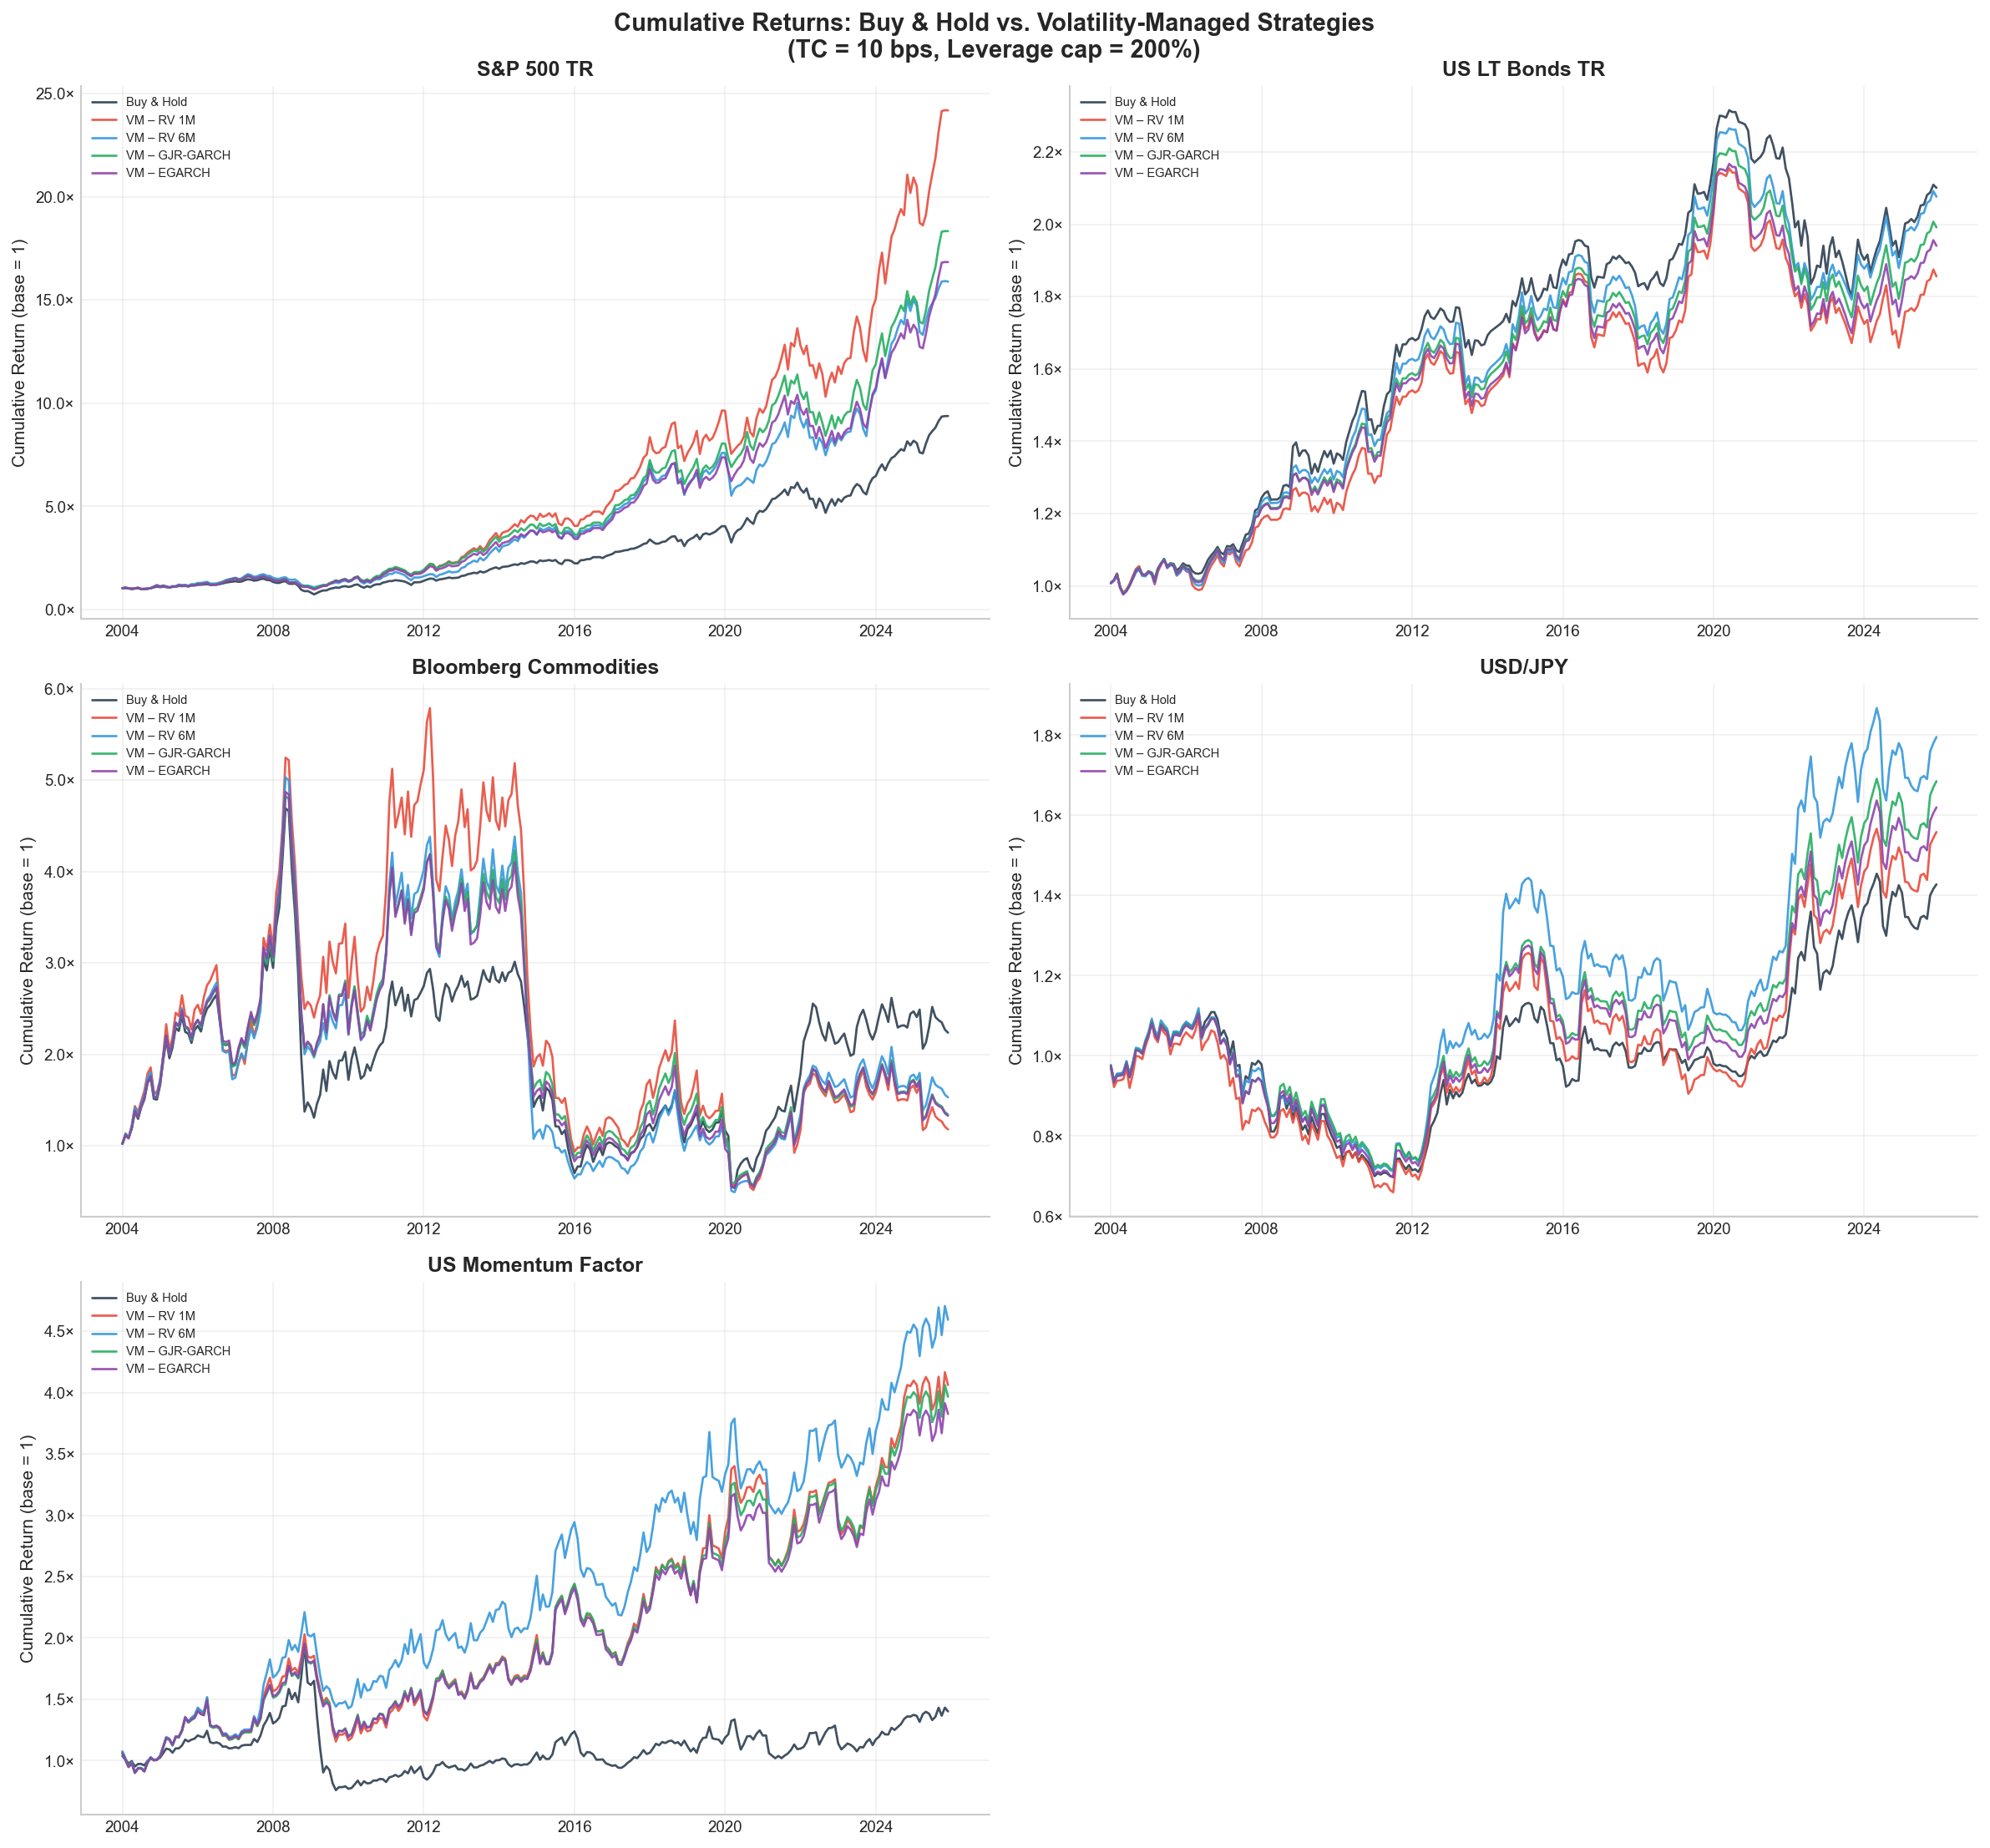
\includegraphics[width=\textwidth]{fig_04_cumulative_returns.png}
  \caption{Cumulative Returns: Buy \& Hold versus Volatility-Managed Strategies
           (TC = 10~bps, Leverage Cap = 200\%). For S\&P~500, VM strategies
           recover sharply post-2009 and post-2020 relative to Buy \& Hold.
           For commodities, VM strategies fail to prevent the secular decline from the
           2008 commodity super-cycle peak ($-$88.5\% drawdown from peak). For USD/JPY,
           RV~6M delivers the strongest outperformance, consistent with the FX
           low-forecastability result.}
  \label{fig:cumulative}
\end{figure}

\subsection{Cross-Asset Executive Summary}

Table~\ref{tab:summary} synthesises the Sharpe ratio differential ($\Delta$Sharpe)
between VM-GJR-GARCH and the Buy-and-Hold benchmark.

\begin{table}[H]
  \centering
  \caption{Executive Summary: Sharpe Ratio Differential ($\Delta$Sharpe = VM-GARCH $-$ B\&H, TC = 10 bps)}
  \label{tab:summary}
  \small
  \begin{tabular}{lccccc}
    \toprule
    \textbf{Asset} & \textbf{B\&H Sharpe} & \textbf{GARCH Sharpe}
                   & \textbf{$\Delta$Sharpe} & \textbf{$\Delta$MaxDD (pp)} & \textbf{Verdict} \\
    \midrule
    S\&P 500 TR          & 0.658 & 0.785 & $+$0.127 & $+$14.1
      & \textcolor{ForestGreen}{\textbf{Strong Add}} \\
    US LT Bonds TR       & 0.294 & 0.256 & $-$0.038 & $+$1.1
      & \textcolor{Red}{\textbf{Neutral/Minus}} \\
    Bloomberg Comm.      & 0.235 & 0.162 & $-$0.073 & $+$0.2
      & \textcolor{Red}{\textbf{Destroys Value}} \\
    USD/JPY              & 0.040 & 0.116 & $+$0.076 & $+$1.7
      & \textcolor{olive}{\textbf{Modest Add}} \\
    US Momentum Factor   & 0.066 & 0.363 & $+$0.297 & $+$22.6
      & \textcolor{ForestGreen}{\textbf{Very Strong Add}} \\
    \bottomrule
  \end{tabular}
  \begin{minipage}{\textwidth}
    \vspace{2pt}
    \footnotesize\textit{Note:} $\Delta$MaxDD = reduction in maximum drawdown in percentage points
    (positive = improvement, i.e., less negative drawdown). GARCH refers to VM-GJR-GARCH.
  \end{minipage}
\end{table}

\subsection{Detailed Discussion of Results by Asset}

\textbf{S\&P 500 (Table~\ref{tab:perf_spxt}).} Volatility management clearly adds value
for US equities. GJR-GARCH raises the Sharpe ratio from 0.658 to 0.785 ($+19.3\%$) and
reduces the maximum drawdown from $-50.9\%$ to $-36.8\%$ --- a 14.1 percentage point
improvement consistent with the findings of \citet{Moreira2017} for US equity factors.
The annualised CAPM alpha of 3.2\% is economically significant. The Sortino ratio
improves dramatically from 0.871 to 1.193, confirming that gains come primarily from
downside risk reduction. RV~1M achieves the highest Sharpe ratio (0.809) but also the
highest turnover (3.73$\times$), making it sensitive to transaction costs. Note that
CAPM beta exceeds 1.0 for all VM strategies, reflecting average leverage above 100\%
consistent with the right-skewed weight distribution in Figure~\ref{fig:weight_dist}.

\textbf{US LT Bonds (Table~\ref{tab:perf_bonds}).} Volatility management modestly destroys
value for government bonds. All VM strategies underperform Buy \& Hold on a Sharpe ratio
basis, with GJR-GARCH reducing the Sharpe from 0.294 to 0.256 ($-13\%$). This result is
consistent with the \emph{flight-to-quality} mechanism: bond volatility spikes during
equity market crises precisely when bonds generate positive returns (negative equity-bond
correlation), so the strategy de-risks at the worst possible moment. The one partial
exception is EGARCH's recession performance (Section~\ref{sec:nber}), which beats Buy \&
Hold on a Sharpe basis during contractions. RV~6M is the least damaging model for bonds
(Sharpe 0.278), owing to its very low turnover (0.68$\times$).

\textbf{Bloomberg Commodities (Table~\ref{tab:perf_comm}).} Volatility management is
counterproductive for commodities ($\Delta$Sharpe $= -0.073$). Two structural factors
drive this result. First, commodities exhibit structurally high base volatility
($\sim$33\%), meaning the strategy spends much of the sample near or at the leverage cap
(mean weight = 1.11, Figure~\ref{fig:weight_dist}), providing limited effective
vol-scaling. Second, the catastrophic drawdown from the 2008 commodity super-cycle peak
($-88.5\%$ over 12 years) is driven by fundamental commodity market dynamics rather than
the vol-clustering shocks that GARCH models anticipate. RV~1M amplifies this problem
by overestimating post-spike volatility, producing the weakest performance (Sharpe 0.175).

\textbf{USD/JPY (Table~\ref{tab:perf_fx}).} A modest improvement is observed
($\Delta$Sharpe $= +0.076$), entirely attributable to the very low base Sharpe of Buy \&
Hold (0.040). RV~6M achieves the best Sharpe (0.142) despite GJR-GARCH dominating on
forecast accuracy; this reflects the weak FX forecastability ($R^2 < 0.30$) and the
consequent benefit of a smooth, low-turnover model that avoids excessive trading costs.
The maximum drawdown is modestly reduced from $-37.1\%$ to $-35.4\%$ under GJR-GARCH.

\textbf{US Momentum Factor (Table~\ref{tab:perf_mom}).} The largest improvement is in
momentum ($\Delta$Sharpe $= +0.297$), corroborating \citet{Moreira2017}'s finding that
vol-scaling momentum is the single most powerful application of the strategy. Momentum
crashes occur precisely during vol spikes (e.g., reversal of March 2009, COVID-19 March
2020), so scaling down automatically during these regimes avoids catastrophic losses. The
reduction in maximum drawdown from $-61.0\%$ to $-38.4\%$ (GARCH) is economically
compelling. Notably, RV~6M achieves the best absolute Sharpe ratio (0.400) and the lowest
turnover (0.80$\times$), making it the preferred implementation for cost-conscious
mandates.

\begin{figure}[H]
  \centering
  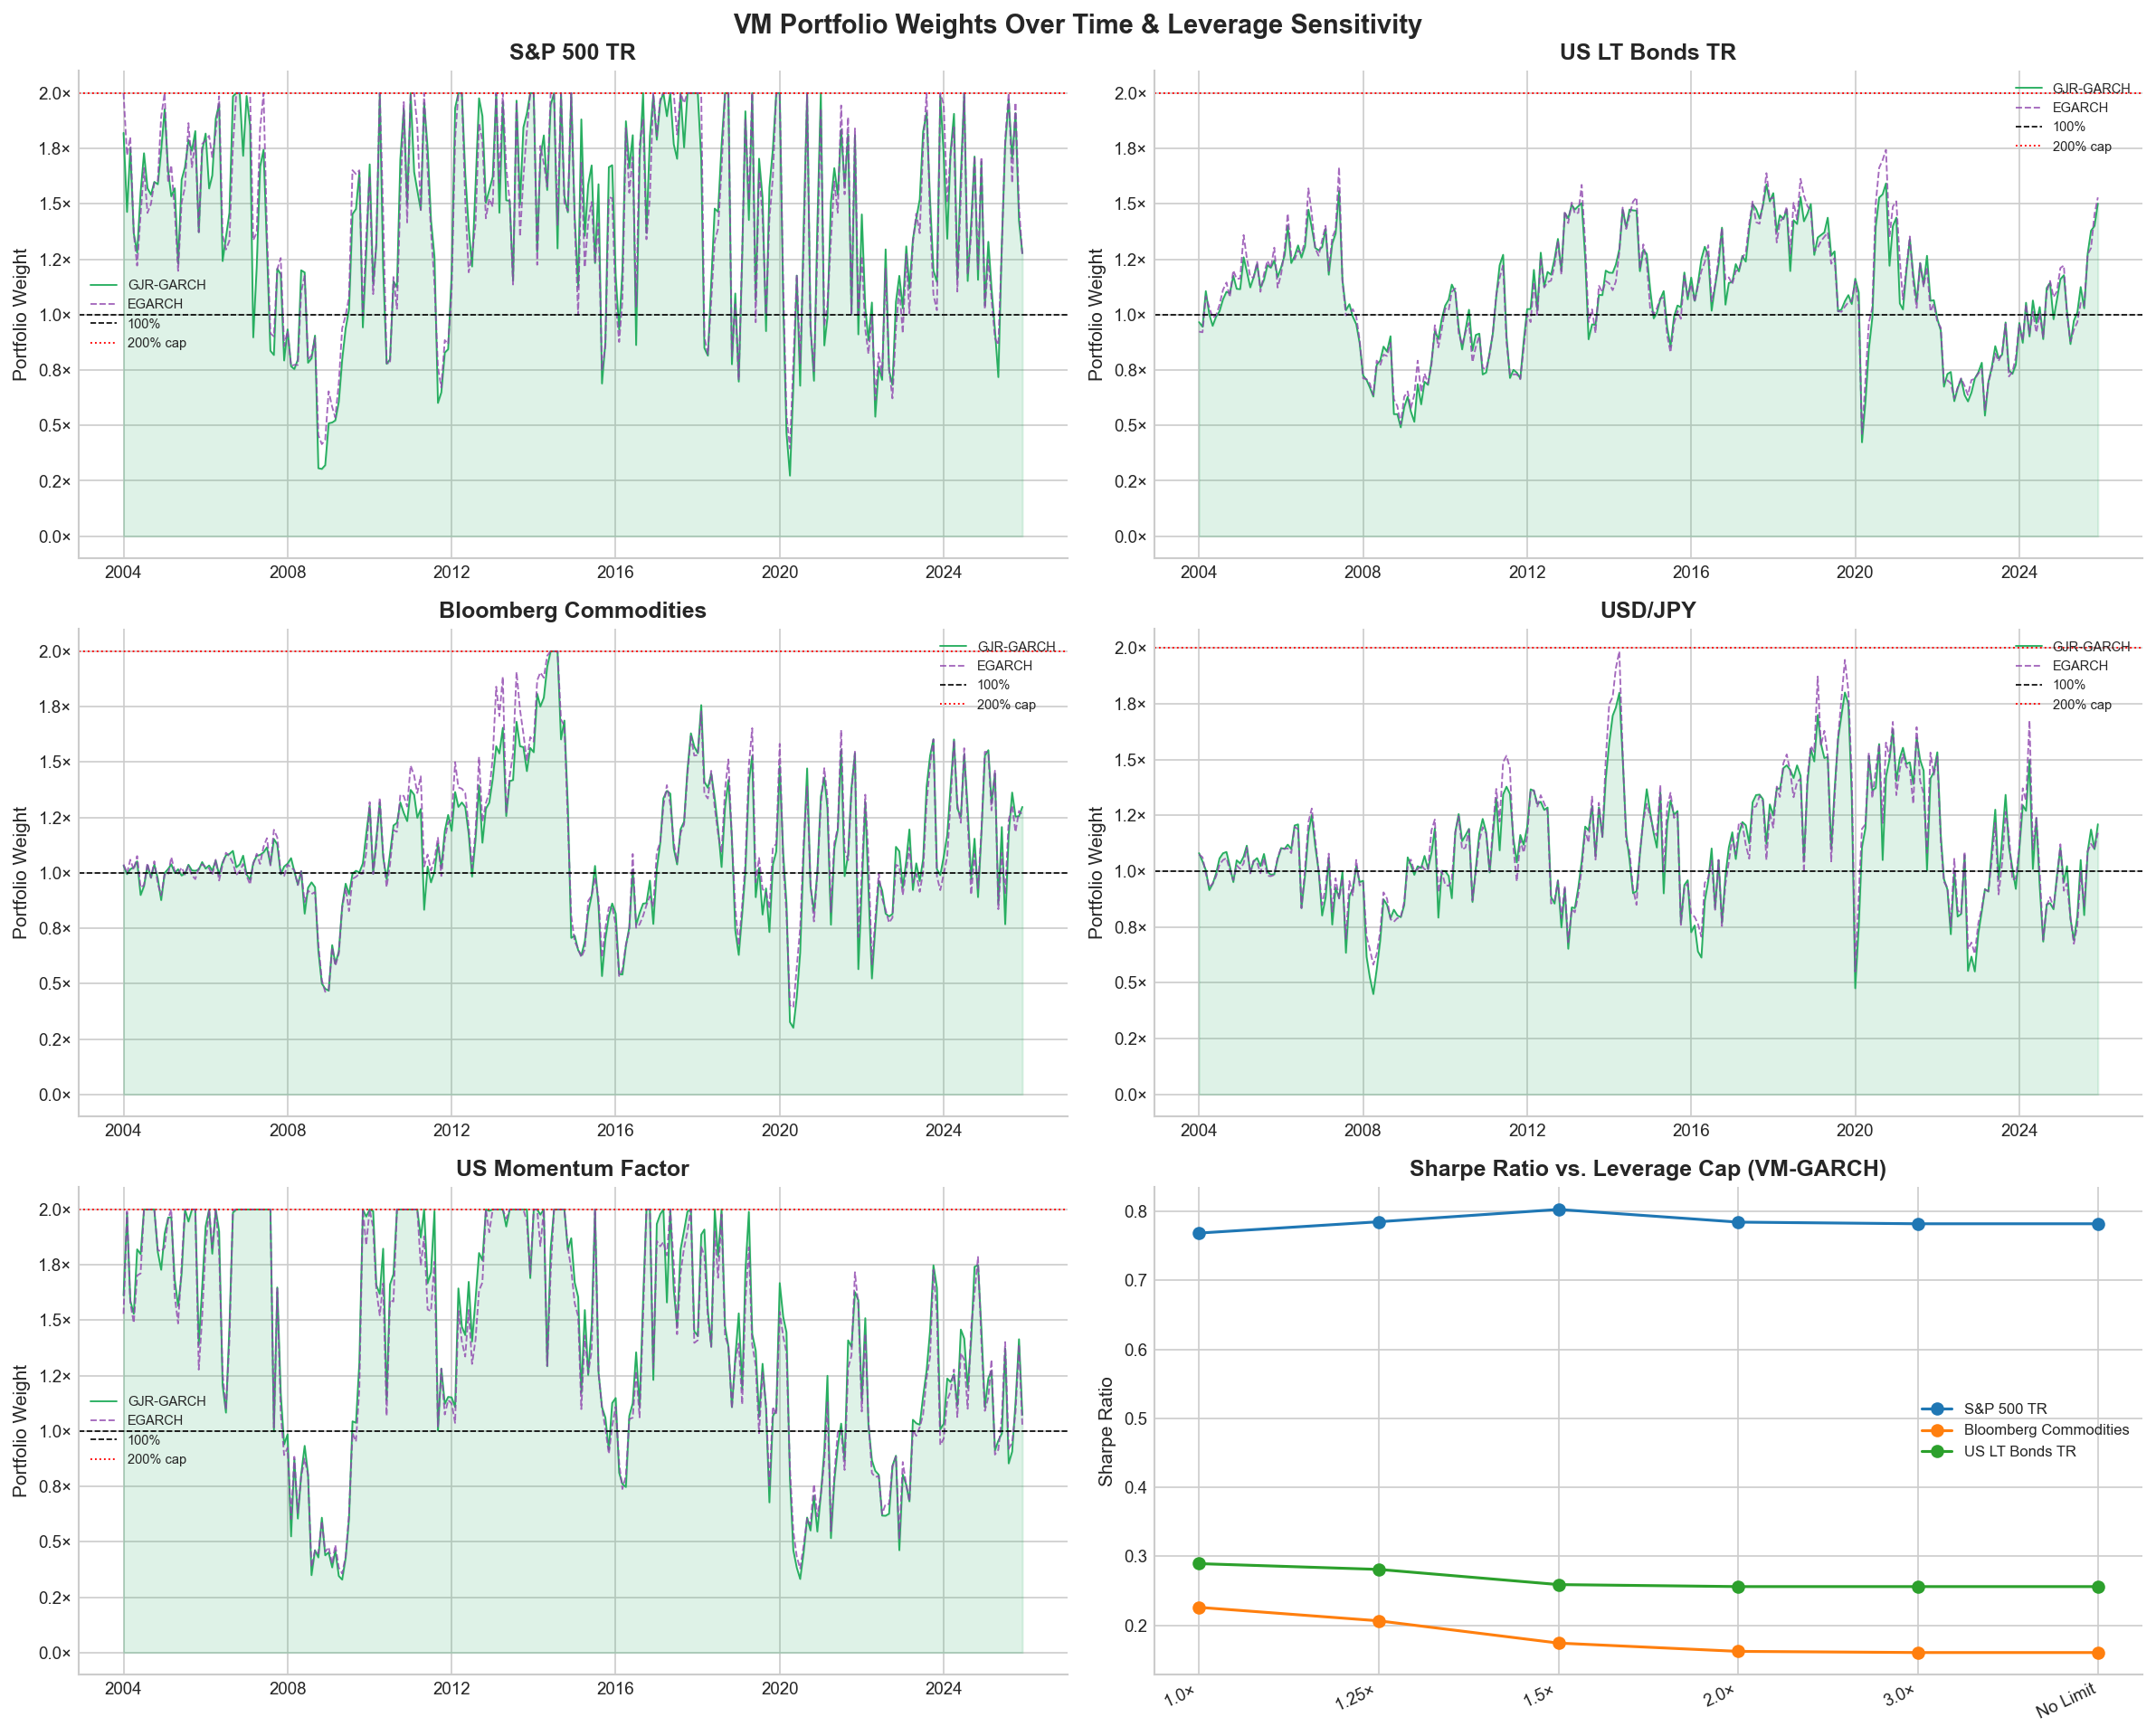
\includegraphics[width=0.9\textwidth]{fig_07_leverage.png}
  \caption{VM Portfolio Weights Over Time (GJR-GARCH and EGARCH, 200\% cap) and Sharpe
           Ratio Sensitivity to Leverage Constraints. For S\&P~500 and Momentum, the cap
           binds frequently in low-volatility regimes (2014--2019, 2021--2023). For US LT
           Bonds, the cap rarely binds (max weight $\leq 1.59\times$). The Sharpe ratio
           for equities is maximised near 1.5× leverage.}
  \label{fig:weights}
\end{figure}

\begin{figure}[H]
  \centering
  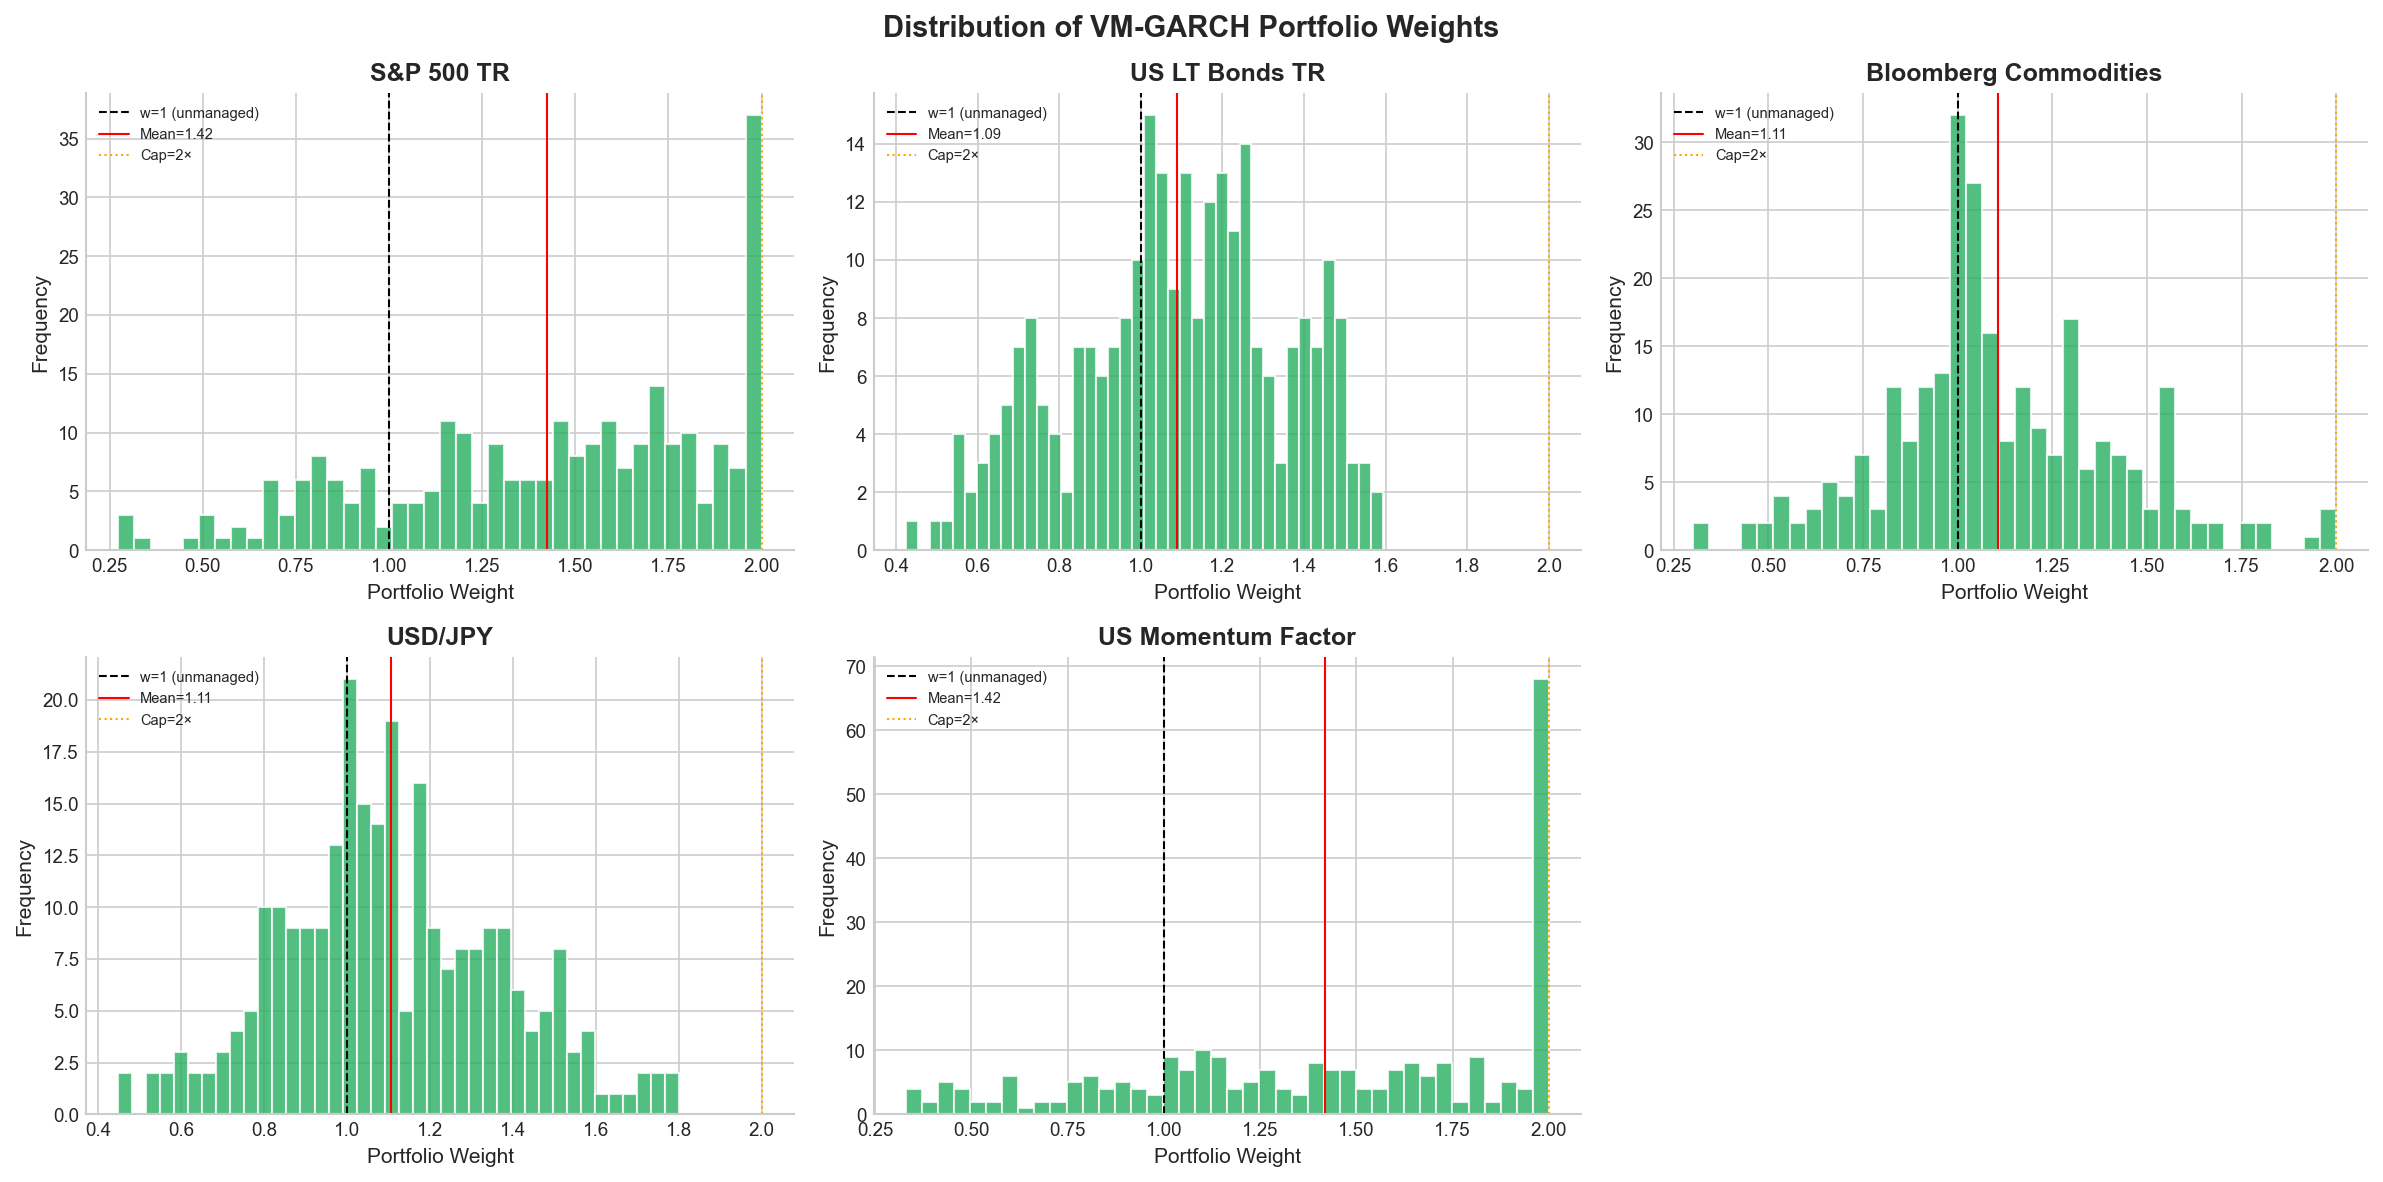
\includegraphics[width=0.85\textwidth]{fig_08_weight_distribution.png}
  \caption{Distribution of VM-GARCH Portfolio Weights across All Assets.
           S\&P~500 and Momentum show strongly right-skewed distributions with a mass at
           the 2× leverage cap (mean weights 1.42 and 1.42 respectively), indicating
           persistent low-volatility regimes. US LT Bonds exhibits a near-uniform
           distribution (mean weight 1.09), consistent with a mean-reverting but
           continuous vol process. Commodities cluster near 1.0× (mean 1.11), consistent
           with their structurally high base volatility relative to the target.}
  \label{fig:weight_dist}
\end{figure}


%% ====================================================================
\section{NBER Business Cycle Analysis}
\label{sec:nber}
%% ====================================================================

A central claim of volatility-targeting proponents is that the strategy provides
\emph{automatic recession hedging}: as volatility spikes in downturns, portfolio weights
mechanically decline. We test this hypothesis using NBER recession dates, following the
same methodology as \citet{Harvey2018}.

\subsection{Recession Periods in the Sample}

Three NBER recessions fall within our 2000--2025 sample:
\begin{enumerate}[noitemsep]
  \item \textbf{Dot-com recession:} March 2001 -- November 2001 (9 months)
  \item \textbf{Great Financial Crisis:} December 2007 -- June 2009 (19 months)
  \item \textbf{COVID-19 recession:} February 2020 -- April 2020 (3 months)
\end{enumerate}
In total, recession months account for 31 of the 312 estimation months (10.0\%). The
GFC dominates in terms of duration and magnitude, creating a sample composition risk:
results may be sensitive to the GFC episode. We therefore note where conclusions are
materially driven by GFC performance.

\subsection{Results by Business Cycle Phase}

Table~\ref{tab:nber} reports annualised returns, volatilities, and Sharpe ratios by
cycle phase. Figure~\ref{fig:nber} provides a visual comparison.

\begin{table}[H]
  \centering
  \caption{Performance by NBER Business Cycle Phase (Annualised)}
  \label{tab:nber}
  \footnotesize
  \begin{tabular}{llcccccc}
    \toprule
    & & \multicolumn{3}{c}{\textbf{Expansion}} & \multicolumn{3}{c}{\textbf{Recession}} \\
    \cmidrule(lr){3-5} \cmidrule(lr){6-8}
    \textbf{Asset} & \textbf{Strategy}
      & \textbf{Ret} & \textbf{Vol} & \textbf{SR}
      & \textbf{Ret} & \textbf{Vol} & \textbf{SR} \\
    \midrule
    \multirow{3}{*}{S\&P 500 TR}
      & Buy \& Hold      & 14.6\% & 12.6\% & 1.16  & $-$25.4\% & 26.5\% & $-$0.96 \\
      & VM -- GJR-GARCH  & 17.7\% & 16.3\% & 1.08  & $-$18.6\% & 16.0\% & $-$1.16 \\
      & VM -- EGARCH     & 17.4\% & 16.1\% & 1.08  & $-$20.6\% & 17.6\% & $-$1.17 \\
    \midrule
    \multirow{3}{*}{US LT Bonds}
      & Buy \& Hold      & 3.1\%  & 6.2\% & 0.50  &  $+$9.0\% & 8.7\% & 1.03 \\
      & VM -- GJR-GARCH  & 3.0\%  & 6.4\% & 0.47  &  $+$6.7\% & 5.9\% & 1.13 \\
      & VM -- EGARCH     & 2.9\%  & 6.5\% & 0.45  &  $+$6.4\% & 6.1\% & 1.05 \\
    \midrule
    \multirow{3}{*}{Bloomberg Comm.}
      & Buy \& Hold      & 15.0\% & 29.0\% & 0.52 & $-$52.4\% & 59.3\% & $-$0.88 \\
      & VM -- GJR-GARCH  & 10.9\% & 31.0\% & 0.35 & $-$35.6\% & 48.6\% & $-$0.73 \\
      & VM -- EGARCH     & 10.9\% & 31.5\% & 0.35 & $-$35.5\% & 47.6\% & $-$0.75 \\
    \midrule
    \multirow{3}{*}{USD/JPY}
      & Buy \& Hold      & 3.1\%  & 9.4\%  &  0.33 & $-$8.7\% & 13.3\% & $-$0.65 \\
      & VM -- GJR-GARCH  & 3.5\%  & 10.2\% &  0.35 & $-$4.3\% & 10.4\% & $-$0.41 \\
      & VM -- EGARCH     & 3.5\%  & 10.2\% &  0.34 & $-$5.4\% & 10.8\% & $-$0.50 \\
    \midrule
    \multirow{3}{*}{US Momentum}
      & Buy \& Hold      & 3.5\%  & 12.0\% & 0.29 & $-$5.7\%  & 34.4\% & $-$0.17 \\
      & VM -- GJR-GARCH  & 7.5\%  & 16.0\% & 0.47 & $+$8.7\%  & 19.5\% & $+$0.45 \\
      & VM -- EGARCH     & 7.3\%  & 15.5\% & 0.47 & $+$7.2\%  & 19.5\% & $+$0.37 \\
    \bottomrule
  \end{tabular}
  \begin{minipage}{\textwidth}
    \vspace{2pt}
    \footnotesize\textit{Note:} Recession months include three NBER recessions (March 2001 -- November 2001;
    December 2007 -- June 2009; February 2020 -- April 2020), totalling 31 months (10.0\% of the
    estimation sample).
  \end{minipage}
\end{table}

\begin{figure}[H]
  \centering
  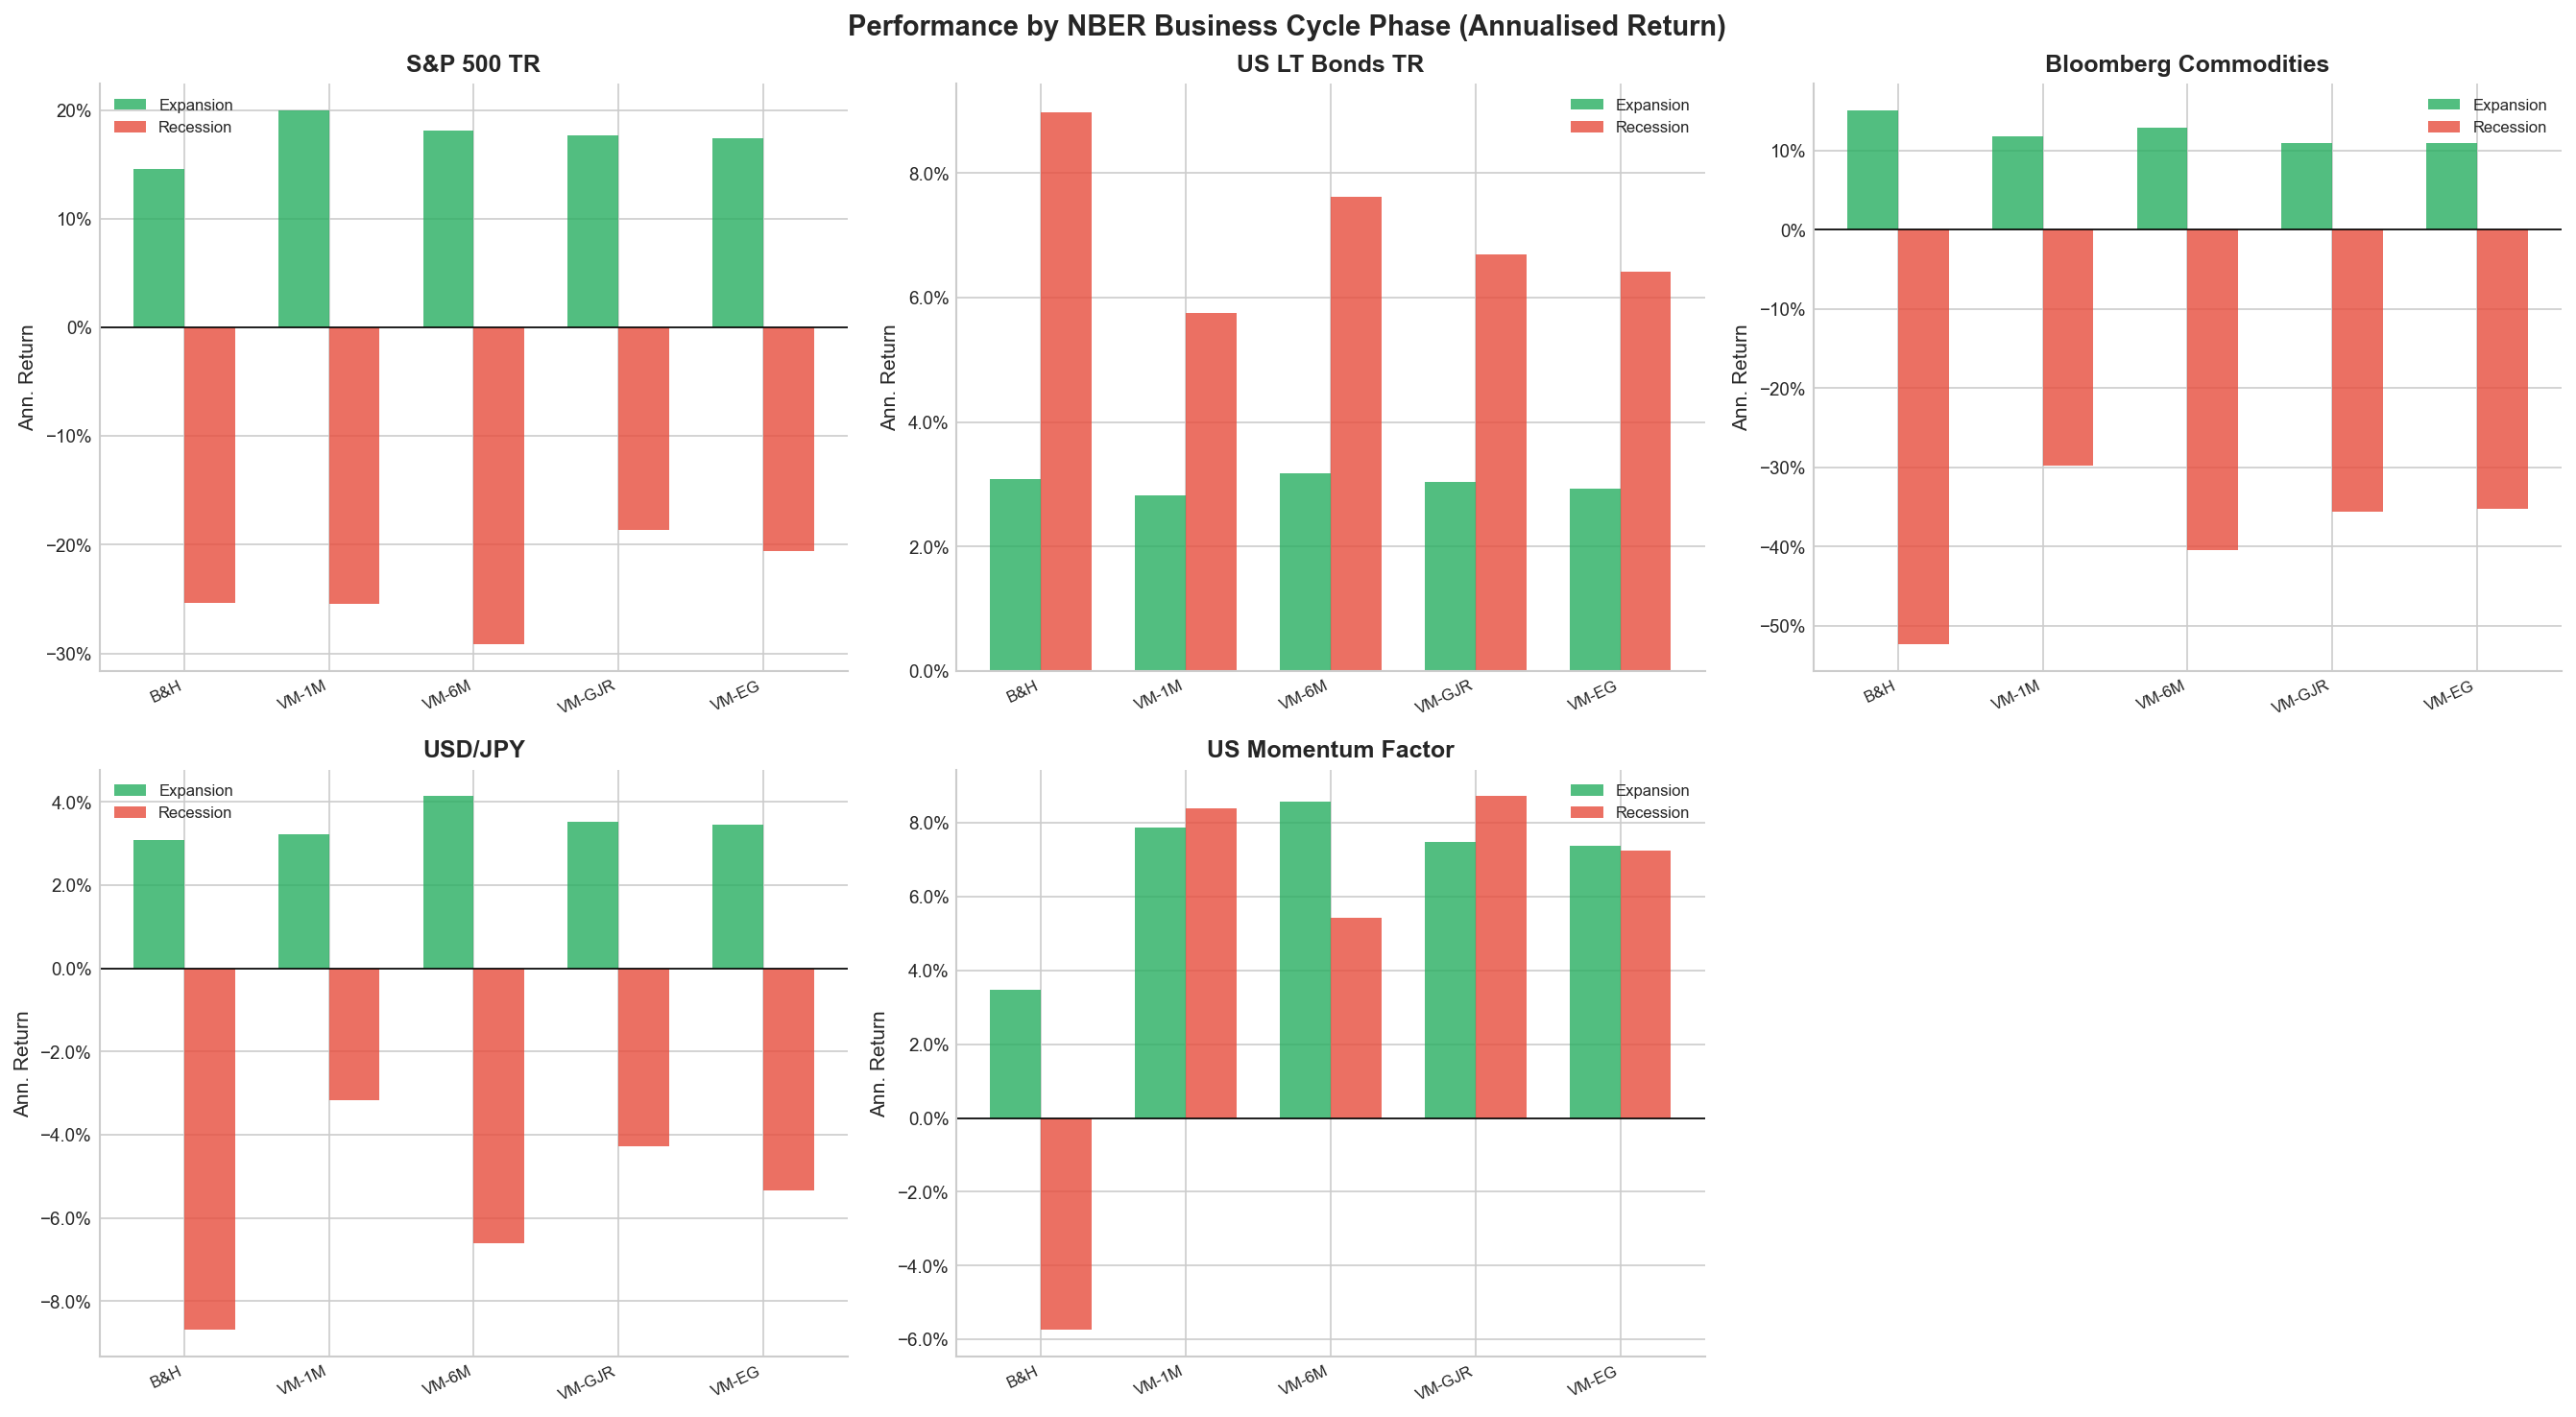
\includegraphics[width=0.95\textwidth]{fig_05_nber.png}
  \caption{Performance by NBER Business Cycle Phase (Annualised Return). VM strategies
           provide meaningful recession protection for S\&P~500 ($+$6.8 pp better than
           B\&H) and dramatically reverse the recession performance of Momentum
           (from $-$5.7\% to $+$8.7\%). For bonds, the flight-to-quality recession premium
           is partially sacrificed by the vol-targeting adjustment.}
  \label{fig:nber}
\end{figure}

\subsection{Discussion}

\textbf{S\&P~500.} VM-GJR-GARCH reduces the recession return loss from $-25.4\%$ to
$-18.6\%$ (annualised), a 6.8 percentage point improvement. Recession volatility falls
from 26.5\% (B\&H) to 16.0\% (VM-GARCH), confirming that the model successfully
de-risks the portfolio as expected during crises. However, the recession Sharpe
ratio ($-1.16$) is \emph{marginally worse} than Buy \& Hold ($-0.96$) because the
higher volatility of the expansion phase (where leverage is used) attracts a higher
tracking error. The economically relevant metric --- absolute dollar loss --- is clearly
superior for VM; the Sharpe comparison in downturns is somewhat misleading when the
portfolio is actively levered in expansions.

\textbf{US LT Bonds.} Bonds exhibit the classic flight-to-quality recession premium: Buy
\& Hold earns $+9.0\%$ (annualised) during recessions versus $+3.1\%$ during expansions.
VM-GARCH, by de-risking when bond vol rises (which often coincides with positive returns
during stress), reduces the recession return to $+6.7\%$ --- partially forgoing this
premium. However, the recession Sharpe under GARCH (1.13) slightly exceeds Buy \& Hold
(1.03) due to proportional volatility compression. This represents a genuine trade-off
for fixed-income investors: VM sacrifices some crisis-return magnitude to reduce vol, but
risk-adjusted performance is marginally better in absolute recession terms.

\textbf{Bloomberg Commodities.} VM strategies meaningfully reduce the recession return
loss from $-52.4\%$ to $-35.6\%$ (GARCH), a 16.8 percentage point improvement. However,
they also sacrifice expansion returns ($+15.0\%$ B\&H vs.\ $+10.9\%$ GARCH), so the
aggregate trade-off remains unfavourable. This confirms that the commodity super-cycle
structural decline is not a vol-clustering shock that can be hedged by vol timing.

\textbf{USD/JPY.} The most notable recession result is the improvement in recession return
from $-8.7\%$ (B\&H) to $-4.3\%$ (VM-GARCH), cutting the recession loss in half.
The reduction in recession volatility from 13.3\% to 10.4\% is also notable. These are
the primary sources of value-add for this asset.

\textbf{US Momentum.} The most striking result: VM-GARCH \emph{turns a negative recession
return} ($-5.7\%$ for B\&H) \emph{into a positive one} ($+8.7\%$). This remarkable
transformation reflects the strategy's capacity to avoid momentum crashes, which are
fundamentally driven by high-volatility regime changes (sudden market reversals). The
expansion Sharpe ratio also improves materially (0.47 vs.\ 0.29 for B\&H). This is the
single most compelling application of volatility-targeting in our dataset.


%% ====================================================================
\section{Transaction Costs, Turnover, and Leverage}
\label{sec:tc}
%% ====================================================================

\subsection{Turnover Analysis}

Table~\ref{tab:turnover} reports annualised turnover for all models and assets.

\begin{table}[H]
  \centering
  \caption{Annualised Turnover by Asset and Forecasting Model (TC = 10 bps)}
  \label{tab:turnover}
  \small
  \begin{tabular}{lcccc}
    \toprule
    \textbf{Asset} & \textbf{VM -- RV 1M} & \textbf{VM -- RV 6M}
                   & \textbf{VM -- GJR-GARCH} & \textbf{VM -- EGARCH} \\
    \midrule
    S\&P 500 TR            & 3.73 & 1.13 & 3.88 & 3.68 \\
    US LT Bonds TR         & 3.06 & 0.68 & 1.19 & 1.19 \\
    Bloomberg Commodities  & 3.50 & 0.78 & 1.78 & 1.77 \\
    USD/JPY                & 3.83 & 0.92 & 1.66 & 1.68 \\
    US Momentum Factor     & 2.80 & 0.80 & 2.42 & 2.35 \\
    \bottomrule
  \end{tabular}
  \begin{minipage}{\textwidth}
    \vspace{2pt}
    \footnotesize\textit{Note:} Turnover = 1.0 means the entire portfolio weight is replaced once per year on average.
    VM--RV~6M achieves the lowest turnover consistently owing to the inherent smoothing of the six-month window.
  \end{minipage}
\end{table}

RV~1M generates the highest turnover (3.73--3.83$\times$ annualised), reflecting its
sensitivity to month-to-month volatility fluctuations. The GARCH models exhibit
intermediate turnover (1.19--3.88$\times$), while RV~6M achieves systematically the
lowest turnover (0.68--1.13$\times$). For S\&P~500, GJR-GARCH's turnover (3.88$\times$)
is marginally higher than RV~1M (3.73$\times$), reflecting more granular monthly variance
updating by the GARCH recursion. For bonds and commodities, GARCH turnover is roughly
half that of RV~1M. The cost of transaction costs at 10~bps for the highest-turnover
model (RV~1M on USD/JPY: 3.83$\times$) amounts to approximately 3.83 $\times$ 10 = 38.3
bps per year --- non-trivial for a low-return asset like USD/JPY.

\subsection{Transaction Cost Sensitivity}

Figure~\ref{fig:tc} and Table~\ref{tab:tc_sensitivity} present the TC sensitivity
analysis. The baseline assumption of 10~bps is consistent with institutional-quality
estimates from \citet{Frazzini2018}, who document one-way transaction costs of 5--20~bps
for large-cap equity futures and ETFs. Our 10~bps baseline is conservative relative to
this range, providing a margin of safety.

\begin{table}[H]
  \centering
  \caption{Transaction Cost Sensitivity: S\&P 500 TR VM-GJR-GARCH vs.\ Buy \& Hold}
  \label{tab:tc_sensitivity}
  \small
  \begin{tabular}{ccccccc}
    \toprule
    \textbf{TC (bps)} & \textbf{B\&H Ret} & \textbf{GARCH Ret} & \textbf{EGARCH Ret}
                      & \textbf{B\&H SR}  & \textbf{GARCH SR}  & \textbf{EGARCH SR} \\
    \midrule
      0  & 10.71\% & 14.58\% & 14.07\% & 0.658 & 0.808 & 0.782 \\
     10  & 10.71\% & 14.14\% & 13.65\% & 0.658 & 0.785 & 0.759 \\
     20  & 10.71\% & 13.70\% & 13.24\% & 0.658 & 0.761 & 0.737 \\
     50  & 10.71\% & 12.40\% & 12.00\% & 0.658 & 0.690 & 0.670 \\
     75  & 10.71\% & 11.32\% & 10.98\% & 0.658 & 0.631 & 0.614 \\
    100  & 10.71\% & 10.25\% &  9.97\% & 0.658 & 0.572 & 0.558 \\
    \midrule
    \multicolumn{3}{l}{\textit{Breakeven TC (GARCH vs.\ B\&H):}}
      & \multicolumn{4}{r}{\textbf{$\approx$ 63.6 bps}} \\
    \bottomrule
  \end{tabular}
\end{table}

\begin{figure}[H]
  \centering
  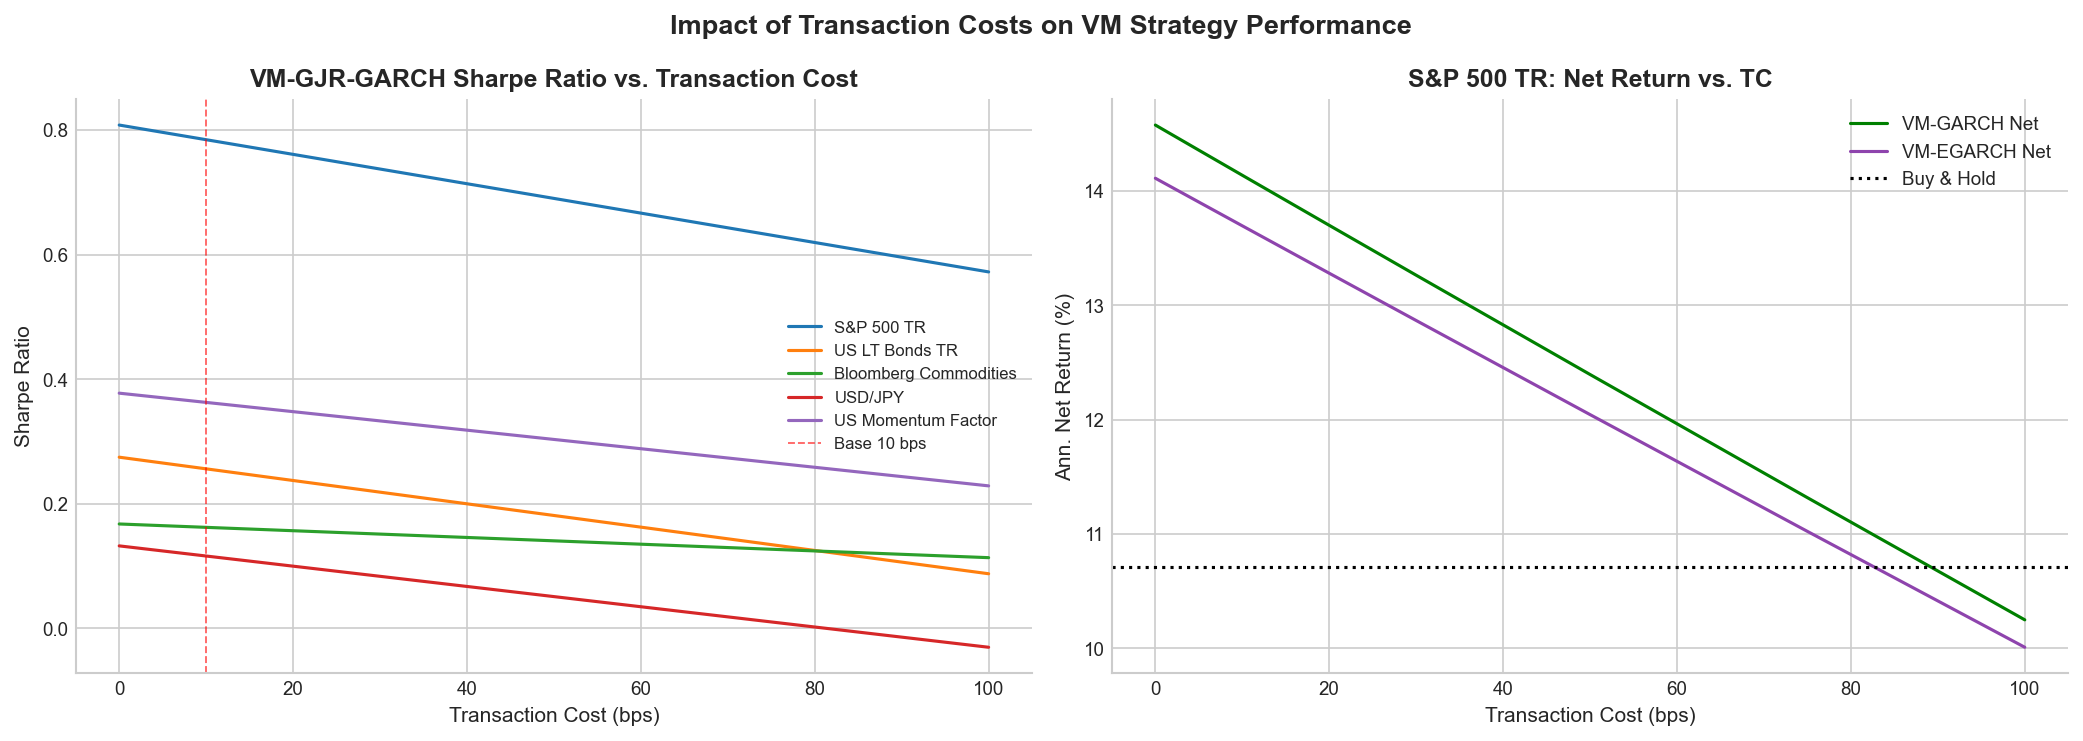
\includegraphics[width=0.92\textwidth]{fig_06_tc_sensitivity.png}
  \caption{Impact of Transaction Costs on VM Strategy Performance.
           \textit{Left:} Sharpe ratio vs.\ TC for all assets (VM-GJR-GARCH); the
           dashed red vertical line marks the 10~bps baseline. \textit{Right:} Net return
           vs.\ TC for S\&P~500 (GARCH and EGARCH vs.\ Buy \& Hold dotted line).
           The breakeven TC for equities is $\approx 63.6$~bps, well above typical
           institutional costs of 10--30~bps.}
  \label{fig:tc}
\end{figure}

The breakeven of $\approx$63.6~bps for the S\&P~500 provides a substantial margin of
safety. At 10~bps, VM-GARCH retains 93\% of its zero-TC net return advantage. At 50~bps
--- a conservative estimate for mid-cap futures or ETF trading in less liquid markets ---
the advantage shrinks to approximately $+1.7\%$ annualised, still positive. Only at
retail-level costs ($\geq 100$~bps) does the strategy fail to outperform Buy \& Hold.
Importantly, the strategy's TC-robustness is a distinguishing feature relative to many
high-turnover factor strategies.

\subsection{Turnover Mitigation Strategies}

We evaluate two turnover-reduction techniques applied to VM-GJR-GARCH:
\begin{itemize}[noitemsep]
  \item \textbf{Threshold banding (Band 10\%):} Rebalance only when $|\Delta w_t| > 10\%$.
        This avoids small weight changes that contribute disproportionately to transaction
        costs relative to their performance benefit.
  \item \textbf{EMA smoothing (span = 3):} Exponentially weighted moving average of
        weights, $\tilde{w}_t = \lambda\,\tilde{w}_{t-1} + (1-\lambda)\,w_t$ with
        $\lambda = 2/(3+1) = 0.5$. This preserves the direction of weight changes while
        dampening their month-to-month magnitude.
\end{itemize}

Table~\ref{tab:mitigation} presents results for all five assets.

\begin{table}[H]
  \centering
  \caption{Turnover Mitigation Strategies: VM-GJR-GARCH (TC = 10~bps)}
  \label{tab:mitigation}
  \small
  \begin{tabular}{llcccc}
    \toprule
    \textbf{Asset} & \textbf{Rule} & \textbf{Ann. Return} & \textbf{Sharpe}
                   & \textbf{MaxDD} & \textbf{Ann.\ Turnover} \\
    \midrule
    \multirow{3}{*}{S\&P 500 TR}
      & Baseline   & 14.1\% & 0.785 & $-$36.8\% & 3.88× \\
      & Band 10\%  & 14.1\% & 0.784 & $-$36.9\% & 3.75× \\
      & EMA span=3 & 14.1\% & 0.761 & $-$39.5\% & 1.84× \\
    \midrule
    \multirow{3}{*}{US LT Bonds}
      & Baseline   & 3.2\%  & 0.256 & $-$21.1\% & 1.19× \\
      & Band 10\%  & 3.3\%  & 0.271 & $-$20.6\% & 0.88× \\
      & EMA span=3 & 3.4\%  & 0.290 & $-$20.8\% & 0.62× \\
    \midrule
    \multirow{3}{*}{Bloomberg Comm.}
      & Baseline   & 1.3\%  & 0.162 & $-$88.3\% & 1.78× \\
      & Band 10\%  & 1.3\%  & 0.160 & $-$87.8\% & 1.56× \\
      & EMA span=3 & 0.7\%  & 0.152 & $-$91.0\% & 0.89× \\
    \midrule
    \multirow{3}{*}{USD/JPY}
      & Baseline   & 2.4\%  & 0.116 & $-$35.4\% & 1.66× \\
      & Band 10\%  & 2.4\%  & 0.120 & $-$35.3\% & 1.45× \\
      & EMA span=3 & 2.4\%  & 0.114 & $-$35.8\% & 0.82× \\
    \midrule
    \multirow{3}{*}{US Momentum}
      & Baseline   & 6.5\%  & 0.363 & $-$38.4\% & 2.42× \\
      & Band 10\%  & 6.3\%  & 0.351 & $-$39.6\% & 2.29× \\
      & EMA span=3 & 6.6\%  & 0.374 & $-$36.8\% & 1.28× \\
    \bottomrule
  \end{tabular}
\end{table}

EMA smoothing reduces turnover by 53\% for equities (3.88$\times$ to 1.84$\times$) and
47\% for momentum (2.42$\times$ to 1.28$\times$), with minimal Sharpe cost ($-0.024$ for
equities) or even improvement ($+0.011$ for momentum, $+0.034$ for bonds). Threshold
banding is less effective for equities (3\% turnover reduction) but achieves 26\% for
bonds (1.19$\times$ to 0.88$\times$) with a Sharpe improvement of $+0.015$. For
commodities, EMA smoothing reduces performance further ($-0.010$ on Sharpe), suggesting
that the faster response of the baseline model provides marginal value in capturing the
rare vol-spike opportunities.

\textbf{Recommendation:} EMA smoothing (span = 3) is the preferred mitigation strategy
for equities and momentum. For bonds, both techniques improve performance, consistent with
the mean-reverting bond vol dynamics where sluggish signals are beneficial.

\subsection{Leverage Sensitivity Analysis}

Table~\ref{tab:leverage} analyses the sensitivity of VM-GJR-GARCH performance to
alternative leverage caps. Figure~\ref{fig:weights} (bottom-right panel) plots Sharpe
ratios against the cap level.

\begin{table}[H]
  \centering
  \caption{Leverage Constraint Sensitivity: VM-GJR-GARCH Sharpe Ratios (TC = 10~bps)}
  \label{tab:leverage}
  \small
  \begin{tabular}{lcccccc}
    \toprule
    \textbf{Asset} & \textbf{1.0×} & \textbf{1.25×} & \textbf{1.5×}
                   & \textbf{2.0×} & \textbf{3.0×} & \textbf{No Limit} \\
    \midrule
    S\&P 500 TR -- Sharpe    & 0.769 & 0.785 & 0.803 & 0.785 & 0.782 & 0.782 \\
    US LT Bonds -- Sharpe    & 0.289 & 0.281 & 0.259 & 0.256 & 0.256 & 0.256 \\
    Bloomberg Comm.\ Sharpe  & 0.226 & 0.206 & 0.174 & 0.162 & 0.160 & 0.160 \\
    USD/JPY -- Sharpe         & 0.071 & 0.091 & 0.105 & 0.116 & 0.116 & 0.116 \\
    \bottomrule
  \end{tabular}
\end{table}

For equities, the Sharpe ratio is maximised at the 1.5$\times$ cap (0.803), marginally
above the 2.0$\times$ baseline (0.785). This reflects the trade-off between capturing
low-vol leverage opportunities and incurring additional rebalancing costs as the cap
boundary is reached and released. Constraining leverage to 1.0$\times$ eliminates
leverage-related TC drag but sacrifices return, reducing equity Sharpe to 0.769.

For bonds and commodities, tighter leverage constraints \emph{improve} risk-adjusted
performance monotonically. For bonds at 1.0$\times$ (Sharpe 0.289 vs.\ 0.256 at
2.0$\times$), this confirms that the additional leverage employed by GARCH does not
generate sufficient return to compensate for its costs. For commodities, capping at
1.0$\times$ (0.226) outperforms by eliminating the structural drag of unnecessary
leveraging in a declining market.

\textbf{Practical implication:} For risk-constrained mandates (variable annuities,
risk-parity structures), a leverage cap of 1.5$\times$ provides the best
risk-adjusted outcome for equities, while limiting operational and margin risk. For
bonds and commodities, capping at 1.0$\times$ (or below) is optimal.


%% ====================================================================
\section{Summary and Recommendations}
\label{sec:summary}
%% ====================================================================

\subsection{Evidence Summary}

This study critically evaluates volatility-targeting strategies across five asset classes
over 25 years (2000--2025), using four forecasting models and a look-ahead-bias-free
implementation following \citet{Bongaerts2020}. The evidence is consistent but nuanced:
\textbf{volatility targeting is not universally beneficial.} Its value depends critically
on four conditions:

\begin{enumerate}
  \item \textbf{Forecast quality:} Strong vol predictability ($R^2 > 0.50$) is a
        necessary condition for material gains; weak predictability (FX, commodities)
        limits performance improvements and renders the strategy sensitive to TC drag.
  \item \textbf{Return-volatility dynamics:} The strategy benefits assets where
        risk-adjusted performance (Sharpe) is inversely related to volatility. Bonds
        violate this assumption during recessions (flight-to-quality), and commodities
        during the super-cycle structural decline.
  \item \textbf{Transaction costs and turnover:} High-frequency models (RV~1M, GARCH)
        generate 3--4$\times$ annualised turnover. The breakeven TC for S\&P~500 is
        $\approx$63.6~bps, providing a generous institutional margin, but turnover-
        mitigation techniques improve the robustness profile.
  \item \textbf{Structural market regimes:} The strategy is particularly effective during
        crisis-and-recovery cycles (GFC 2008--2009, COVID-19 2020) but adds limited
        value in secular trends such as the commodity super-cycle decline.
\end{enumerate}

\subsection{Recommendations to the Volatility Management Board}

\paragraph{Recommendation 1 --- Adopt for Equities (S\&P~500 TR).} VM-GJR-GARCH generates
a robust Sharpe improvement of $+0.127$ ($+19.3\%$) and reduces maximum drawdown from
$-50.9\%$ to $-36.8\%$ at 10~bps TC. The breakeven cost ($\approx$63.6~bps) provides
ample margin of safety. \textit{Preferred model: GJR-GARCH with EMA smoothing (span = 3)
and leverage cap of 1.5$\times$.}

\paragraph{Recommendation 2 --- Adopt for Momentum (MOM).} The improvement is the largest
across all assets ($\Delta$Sharpe $= +0.297$). The NBER analysis demonstrates that the
strategy even generates \emph{positive} returns during recessions (GJR-GARCH: $+8.7\%$)
versus Buy \& Hold's $-5.7\%$. This is the single most compelling application of
volatility-targeting in our dataset. \textit{Preferred model: VM-RV~6M (Sharpe 0.400,
lowest turnover at 0.80$\times$) or VM-GJR-GARCH with EMA smoothing.}

\paragraph{Recommendation 3 --- Do Not Adopt for Commodities.} Volatility management
consistently destroys value for the Bloomberg Commodity Index across all four models
($\Delta$Sharpe ranges from $-0.040$ to $-0.073$). The structural combination of high
base volatility, weak forecast quality ($R^2 < 0.42$), and a secular commodity price
decline creates an environment where vol-targeting provides no edge. We recommend managing
commodity risk through position sizing and cross-asset diversification rather than
volatility targeting.

\paragraph{Recommendation 4 --- Do Not Adopt for Bonds.} The flight-to-quality mechanism
means bond volatility spikes coincide with positive return episodes. VM strategies, by
de-risking at these moments, sacrifice a structural risk premium. The $\Delta$Sharpe of
$-0.038$ (GARCH) is modest but consistent across all four models. The one mitigating
factor is the marginal improvement in recession Sharpe (1.13 for GARCH vs.\ 1.03 for
B\&H), which may appeal to liability-driven investors seeking smoother cycle performance
at the cost of some crisis upside.

\paragraph{Recommendation 5 --- Marginal Adoption for USD/JPY.} The improvement is
positive but modest ($\Delta$Sharpe $= +0.076$). Given the structurally weak
forecastability of FX volatility, the strategy adds value primarily by moderating the
drawdown from $-37.1\%$ to $-35.4\%$. \textit{Preferred model: VM-RV~6M (Sharpe 0.142)
due to lowest turnover and best absolute performance.}

\paragraph{Recommendation 6 --- Model Selection.} For all adopted strategies, GJR-GARCH
is the preferred primary model on three grounds: (i) superior RMSE and $R^2$ for equities
and momentum; (ii) the leverage-effect mechanism ($\gamma > 0$) is economically
interpretable and empirically robust; and (iii) the DM test finds no significant accuracy
difference vs.\ EGARCH, but GJR-GARCH consistently generates higher net portfolio Sharpe
for equities. EGARCH serves as a robustness check and may be preferred for bonds and
commodities on forecast-accuracy grounds.

\paragraph{Recommendation 7 --- Turnover and Leverage Controls.} We recommend EMA
smoothing (span = 3) for equities and momentum, reducing turnover by $\approx$50\% with
negligible Sharpe cost. Leverage should be capped at 1.5$\times$ for equities and
1.0$\times$ for all other adopted assets. These implementation choices preserve
essentially all of the strategy's risk-adjusted performance advantage while significantly
improving implementation robustness.

\subsection{Limitations and Future Research}

Several limitations merit acknowledgement. First, the sample (2000--2025) is dominated by
two major crises and an extended low-rate environment; the strategy's value-add over a
shorter or different window may differ from full-sample results \citep{Liu2019}. Second,
daily rebalancing within each month is assumed, which may not reflect operational
constraints of real-world implementation. Third, the transaction cost model is simplistic
(linear, one-way); market impact and bid-ask spreads are likely non-linear for large
positions. Fourth, we use a single-asset framework; multi-asset volatility-targeting with
dynamic correlation adjustments (as in \citealt{Bongaerts2020}) remains an important
avenue for future work. Finally, the momentum factor is sourced from the Fama-French
library at a specific construction methodology; alternative momentum definitions
(e.g., risk-adjusted momentum) may alter conclusions.


%% ====================================================================
%% ====================================================================

\begin{thebibliography}{99}

\bibitem[Andersen et al.(2003)]{Andersen2003}
Andersen, T.~G., Bollerslev, T., Diebold, F.~X., \& Labys, P. (2003).
Modeling and forecasting realized volatility.
\textit{Econometrica}, 71(2), 579--625.

\bibitem[Bongaerts et al.(2020)]{Bongaerts2020}
Bongaerts, D., Kang, X., \& van Dijk, M. (2020).
Conditional volatility targeting.
\textit{Financial Analysts Journal}, 76(4), 54--71.

\bibitem[Diebold \& Mariano(1995)]{DM1995}
Diebold, F.~X., \& Mariano, R.~S. (1995).
Comparing predictive accuracy.
\textit{Journal of Business \& Economic Statistics}, 13(3), 253--263.

\bibitem[Frazzini et al.(2018)]{Frazzini2018}
Frazzini, A., Israel, R., \& Moskowitz, T.~J. (2018).
Trading costs.
\textit{Working Paper, AQR Capital Management}.

\bibitem[Glosten et al.(1993)]{Glosten1993}
Glosten, L.~R., Jagannathan, R., \& Runkle, D.~E. (1993).
On the relation between the expected value and the volatility of the nominal excess
return on stocks.
\textit{Journal of Finance}, 48(5), 1779--1801.

\bibitem[Harvey et al.(2018)]{Harvey2018}
Harvey, C.~R., Hoyle, E., Korgaonkar, R., Rattray, S., Sargaison, M., \&
Van Hemert, O. (2018).
The impact of volatility targeting.
\textit{Journal of Portfolio Management}, 45(1), 14--33.

\bibitem[Liu et al.(2019)]{Liu2019}
Liu, F., Tang, X., \& Zhou, G. (2019).
Volatility-managed portfolio: Does it really work?
\textit{Journal of Portfolio Management}, 46(1), 38--51.

\bibitem[Meese \& Rogoff(1983)]{Meese1983}
Meese, R.~A., \& Rogoff, K. (1983).
Empirical exchange rate models of the seventies: Do they fit out of sample?
\textit{Journal of International Economics}, 14(1--2), 3--24.

\bibitem[Mincer \& Zarnowitz(1969)]{Mincer1969}
Mincer, J., \& Zarnowitz, V. (1969).
The evaluation of economic forecasts.
In J. Mincer (Ed.), \textit{Economic Forecasts and Expectations} (pp.~1--46). NBER.

\bibitem[Moreira \& Muir(2017)]{Moreira2017}
Moreira, A., \& Muir, T. (2017).
Volatility-managed portfolios.
\textit{Journal of Finance}, 72(4), 1611--1644.

\bibitem[Nelson(1991)]{Nelson1991}
Nelson, D.~B. (1991).
Conditional heteroskedasticity in asset returns: A new approach.
\textit{Econometrica}, 59(2), 347--370.

\end{thebibliography}

\end{document}
